\chapter{Experiments} \label{ch:experiments}
In this chapter, first the notion of a registration error metric is looked at in more detail, and then the limits of the accuracy of the \gls{icp} algorithm is analyzed. For this a series of experimental \gls{icp} registrations are run with different inputs, and the results are compared.

\section{Evaluation of registration accuracy}
The output of any registration algorithm that aligns a loose point clouds $Q$ with a fixed point cloud $P$ is a rigid transformation matrix $\matr{\hat{M}}$, or possibly an indication that the algorithm has failed. In the ideal case, which is not reachable in practice, it will be equal to the \emph{true} transformation $\matr{M}$.

In order to evaluate the result, it is useful to have a numerical metric $e(\matr{\hat{M}})$ that indicates the ``accuracy'' of  $\matr{\hat{M}}$, both for the cases when the true transformation is known and when it is unknown. It should be minimal when $\matr{\hat{M}} = \matr{M}$, and it should indicate a spatial distance.

\subsection{Known true transformation} \label{sec:lm_known_ttrans}
When $\matr{M}$ is known, the accuracy is measured by how much $\matr{\hat{M}}$ deviates from $\matr{M}$. The rigid transformation, relative to the true transformation, is given by $\matr{\hat{M}}_{\text{rel}} = \matr{M} \matr{\hat{M}} \matr{M}^{-1}$.

Using $\matr{\hat{M}}_{\text{rel}}$, one can calculate for each point $q \in Q$ the \emph{true} correspondence point $q' = \matr{\hat{M}}_{\text{rel}}^{-1} \, \vec{q}$. It is the position in $P$ that corresponds to $q \in Q$. Unless $P$ and $Q$ have the exact same constellation of points, there is generally no point $p \in P$ that coincides with this $q'$. The knowledge of $\matr{M}$ is used to simulate the existence of $P$ with exactly the same constellation.

As a metric for the accuracy of $\matr{\hat{M}}$, the average of the unsigned distances between $q$ and $q'$ is used:
\begin{equation}
e(\matr{\hat{M}}) = \frac{1}{n} \, \sum_{i=1}^{n} \| q_i - q'_i \|
\end{equation}
This metric will be called the \emph{true error}. It is similar to the ICP point-to-point (mean square error) error metric, just with the real correspondences, and without squaring the terms. Using a point-to-plane or other metric would not be useful because the correspondences are exact.

When $\matr{\hat{M}} = \matr{M}$, the absolute minimum $e(\matr{\hat{M}}) = 0$ is reached, as all points $q = q'$ coincide. When $\matr{M}$ is only a translation $\vec{t}$, $e(\matr{\hat{M}}) = \| \vec{t} \|$. When a small rotation with center $\vec{0}$ (the origin $Q$) is added, all points $q$ move away from $q'$ in a circular motion. Using trigonometric approximation for small angles, this length of movement is proportional to $\| q, \vec{0}\|$, and not to the squared distance. Hence taking the average of unsigned distances $q - q'$ can give a useful value.

\subsection{Unknown true transformation}
When the true transformation $\matr{M}$ is unknown, no exact metric for the accuracy of the registration can be defined. It is not known for which input value any such error metric $e$ should reach its minimum. Deciding whether the registration is accurate enough ultimately needs some heuristics, such as a human checking whether the point clouds visually appear well enough aligned for their intended purpose.

The point-to-point or other error metrics used by \gls{icp} depend on the estimated point correspondences, and attain local minima for values of $\matr{M}$ where the estimated correspondences are incorrect, but the average distance is low. Also the correspondence selection needs to be adjusted in function of the occlusions, different bounds and densities of $P$ and $Q$. An error metric calculated from one-on-one point correspondences is necessarily limited by which points are available in $P$ and $Q$. Techniques such as point-to-plane \gls{icp} and generalized ICP try to infer information about the local shape of the surface around a point.

Point-to-point \gls{icp} uses a mean squared error, which allows for least squares error minimization. When the goal is just to evaluate the accuracy of a supposed registration, the \emph{mean absolute error} can be more useful. It is the average of the unsigned distances between each point $q$ and its estimated corresponding point in $p$.
\begin{equation}
e(\matr{\hat{M}}) = \frac{1}{n} \, \sum_{i=1}^{n} \| q_i - p_i \|
\end{equation}
This way the error metric approximates the one defined above for the true correspondences.


\subsection{Visualization of error metric} \label{sec:err_vis}
The rigid transformation matrix $\matr{M}$ has $6$ degrees of freedom: three axis of translation and three angles of rotation. Both the translation and the rotation cannot be represented in a continuous way using less than $3$ real numbers. A natural way to map $6$ real numbers to a rigid transformation is to use a fixed orthonormal coordinate system, and use three values as components for the translation vector, and three values as Euler angles for the rotation.

So an error metric $e(\matr{\hat{M}}_{\text{rel}})$ is a function from $\mathbb{R}^6$ to $\mathbb{R}$. For a good error metric it can be expected that $e(\matr{M}) \approx 0$, and the area around $\matr{M}$ is of interest to evaluate the registration accuracy. It cannot be visualized directly as a six-dimensional density plot, so a way to approximate it is to use two- or one-dimensional cross-sections instead.

An easy way to generate a one-dimensional cross section plot is to fix $5$ components and record the values of $e(m)$ as one component varies. But this is biased towards the axis of the used coordinate system, which are typically irrelevant to the point cloud. A more useful way is to take a random rigid transformation $\matr{M'}$, and gradually interpolate from $\matr{M}$ to $\matr{M'}$.

As shown in section \ref{sec:rot_interp} a linear interpolation between two rigid transformations can be constructed by linearly interpolating the translation vector components, and calculating the \emph{slerp} for the rotational interpolation. Here an interpolation function $i(t, \matr{M'})$ is constructed based on this, with $t \in [-1, +1]$. It is such that $i(-1, \matr{M'}) = (\matr{M'})^{-1}$, $i(0, \matr{M'}) = \matr{M}$ and $i(+1, \matr{M'}) = \matr{M'}$.

$\matr{M'}$ is decomposed into the translational part and the rotational part, both are interpolated as described, and then again composed into a rigid transformation. The negative part needs to be handled separately because the slerp is only defined for $t \in [0, 1]$.

For choosing a random rigid transformation, an angular magnitude $\theta$ and a translational magnitude $m$ are first fixed. Then two random unit vectors $\vec{t}$ and $\vec{\omega}$ are chosen, according to a uniform probability distribution. The resulting rigid transformation is the composition of the translation $m \vec{t}$, and the rotation around axis $\vec{\omega}$ by angle $\theta$. Both $m$ and $\theta$ can always be taken as positive values, since rotation in the other direction takes place when $\vec{\omega}$ points in the opposite direction. When $\theta = r m$ (in radiants), it will move on a sphere of radius $r$ centered at the point cloud origin, by the same amount as it moves on the translation axis. So it makes sense to fix $r$ in function of the size and shape of the model.

Now a visualization of an error metric is created by first choosing $n$ random rigid transformations $\matr{M}_i$, and then plotting $e(i(t, \matr{M}_1)), \cdots, e(i(t, \matr{M}_n))$ against $t \in [-1, +1]$, on the same graph. A similar approach for visualizing error metrics is for instance used by \cite{Boua2013}.

An example of a graph generated this way is shown on figure \ref{fig:mea_plot}. It shows the \emph{mean absolute error} error metric measured on a point cloud, with correspondences established using the closest point criterion.

\begin{figure}[h]
\centering
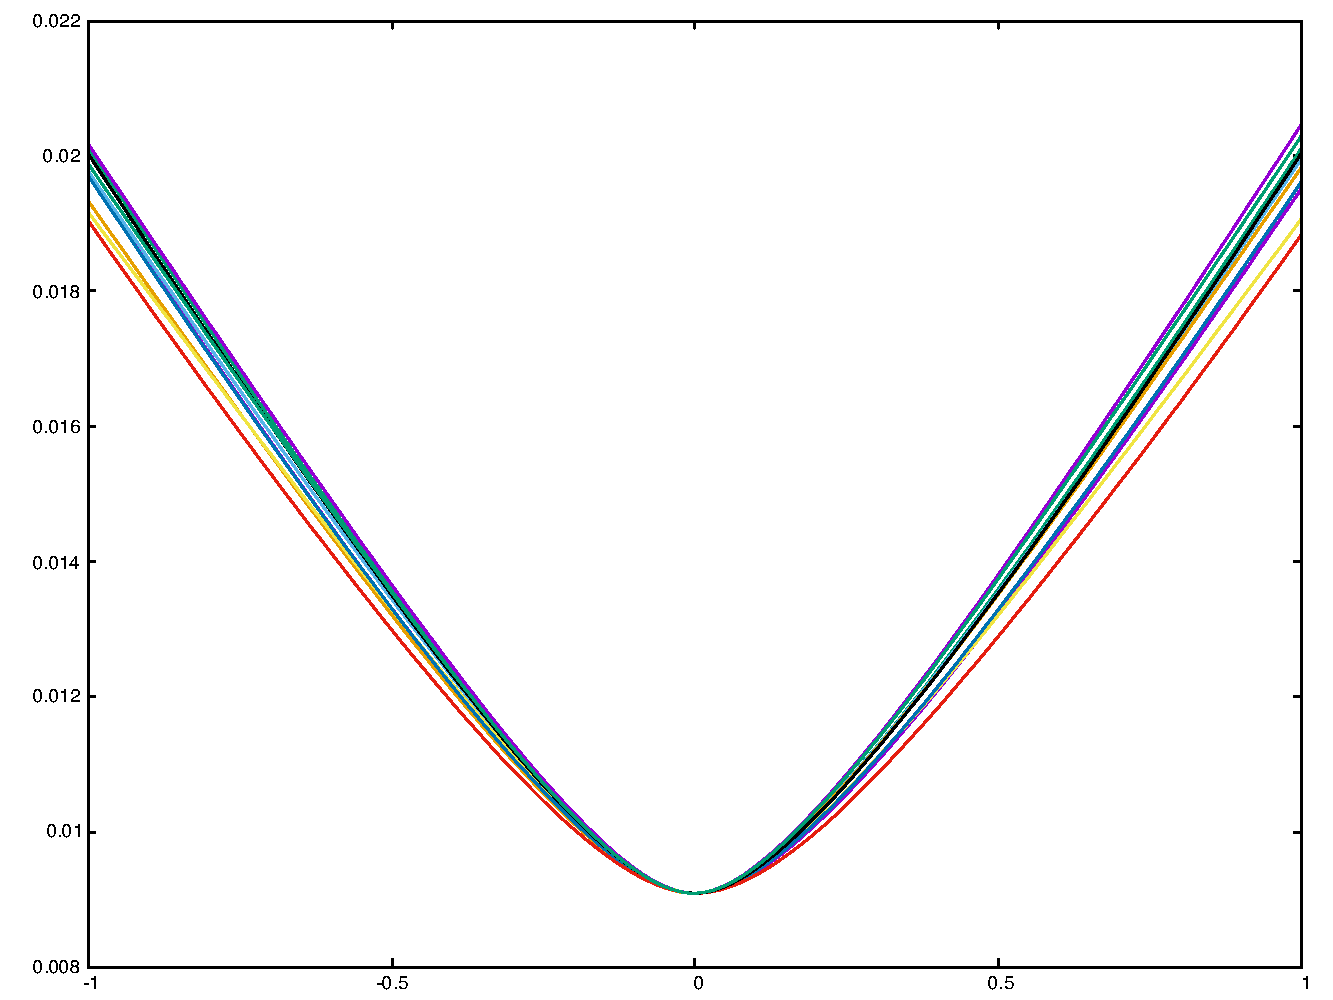
\includegraphics[width=.5\textwidth]{fig/mea_plot.pdf}
\caption{Multi-axis visualization of mean absolute error metric}
\label{fig:mea_plot}
\end{figure}

Because multiple interpolation axis (or planes) cannot easily be visually overlapped, two-dimensional plots of the error function are less useful, unless the two chosen axis have a special significance. For example if they are the translation axis which span the plane of an approximatively planar model.


\newpage



\section{ICP registration experiments} \label{sec:icp_reg_exp}
Some experiments were run with the \gls{icp} algorithm with different artificial point clouds as input in order to determine how accurately they can be registered with it. The true transformation $\matr{M}$ is known, but \gls{icp} only uses an estimated error metric. After running \gls{icp} on the point clouds, it is tested how closely the final estimated transformation is to $\matr{M}$, that is, how small the \emph{true error} metric of the estimated transformation is.

Because the aim is not to study the convergence evolution of \gls{icp}, but rather the accuracy of the final registration, in most of the test runs the point clouds will be perfectly aligned initially. After registration with \gls{icp} they tend to diverge from this true transformation by a small amount. Two cases are studied: (1) The two point clouds have different resolutions, and (2) They have different camera view poses resulting in low overlap.

For these experiments only the most basic variant of \gls{icp} has been used, with a point-to-point error metric and the closest point criterion. The software framework implemented to conduct the experiments will be described in chapter \ref{ch:implementation}.

When attempting to register a short-range scan of a relatively small object with the same object in a long-range scan, the short-range point cloud will have a much higher resolution. But fine registration algorithms generally make the assumption that the two point clouds have similar resolutions. The issue of registering point clouds with different resolutions seems to be largely ignored in the literature about point cloud registration algorithms.

\subsection{Different resolutions experiment}
A first observation is that in general for \gls{icp}, lowering the resolution of the loose point cloud does not much reduce the accuracy of the registrations. This is shown in the following experiment. The Stanford Bunny model is fine registered with a lower density copy of itself. Let $P$ be the fixed point cloud and $Q$ the (downsampled) loose point cloud.

The most basic variant of \gls{icp} is used: All points are selected, correspondences from are taken $Q$ to $P$ by the closest point criterion, no correspondences are rejected, weights are uniform, and the point-to-point error metric is used. The copies are made in such a way that they never have two points in common: $P$ is constructed by taking randomly chosen $50\%$ of the points from the original model, and $Q$ is constructed from the remaining $50\%$. After this $Q$ is randomly downsampled by $60$ different amounts.

The experiment is done in three instances. For the first one (figure \ref{fig:bunny_globmin}), $P$ and $Q$ start out perfectly aligned, and for the two other ones (figures \ref{fig:bunny_globsmall} and \ref{fig:bunny_globmed}), they start out with a small (or larger) random initial transformation. $40$ iterations of the registration algorithm are run and the final errors are recorded.

The plots show the \emph{true error}, as defined in section \ref{sec:lm_known_ttrans}. It is zero if and only if $P$ and $Q$ are perfectly aligned. The X axis indicates the ratio of the number of points $\frac{\|Q\|}{\|P\|}$.

\begin{figure}[H]
\begin{tabularx}{\textwidth}{|r|X|} \hline
Method & ICP. Select all points, closest point criterion, equal weights, no rejection, point-to-point error metric. \\ \hline
Model & Stanford Bunny model. \\ \hline
Fixed ($P$) & 50\% of model points, randomly chosen. \\ \hline
Loose ($Q$) & Starting from the other 50\%, randomly downsampled by given amount. $60$ steps. \\ \hline
Displacement & See captions on the figures. \\ \hline
Y Axis & True error, after $40$ iterations. \\\hline
X Axis & Number of points in Loose divided by number of points in Fixed. Lower value means Loose has lover resolution. \\ \hline
\end{tabularx}
\end{figure}

\subsubsection{No displacement}
The two point clouds are perfectly aligned to start with.

\begin{figure}[H]
\centering
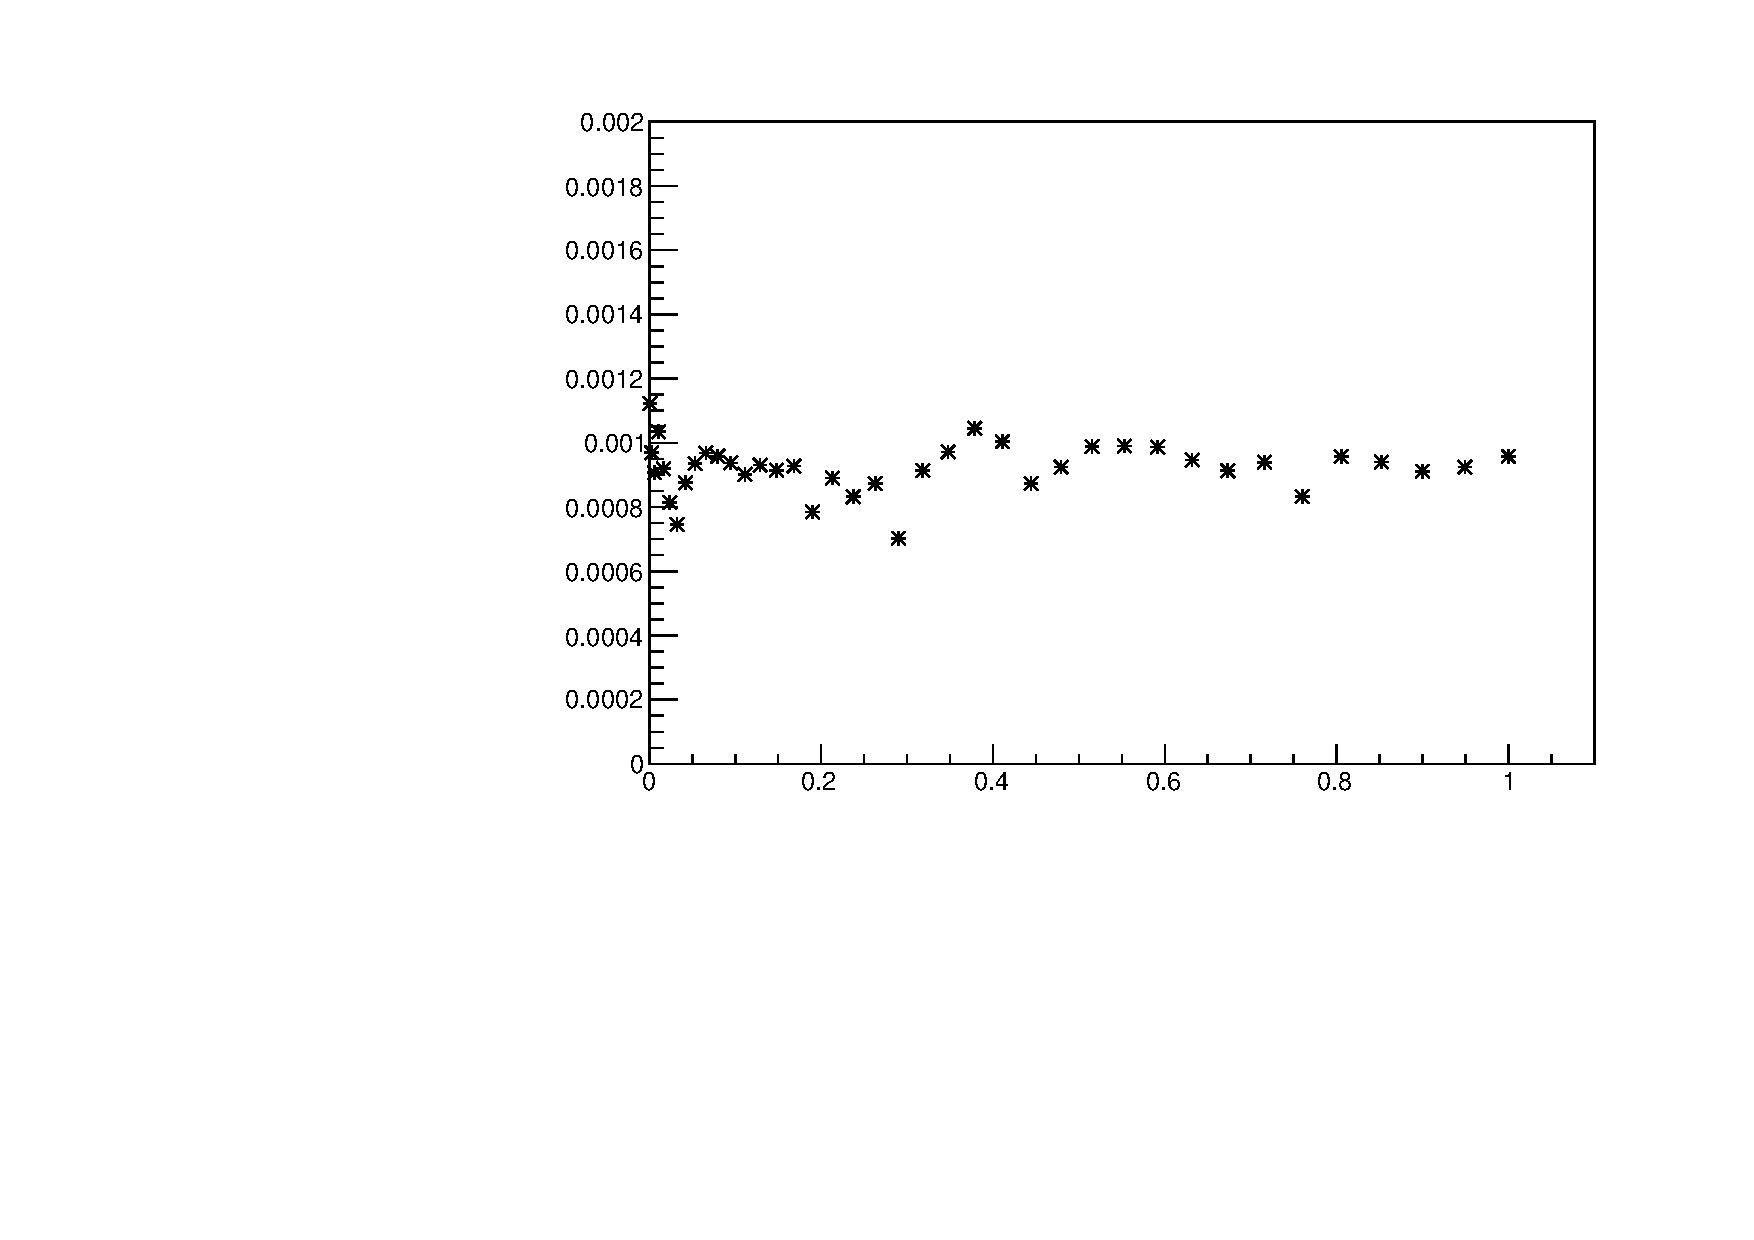
\includegraphics[width=.7\textwidth]{fig/bunny_globmin.pdf}
\caption{no displacement}
\label{fig:bunny_globmin}
\end{figure}

\subsubsection{Small displacement}
Small displacement. Translation by magnitude of $0.01$ in random direction, rotation by $3 \si{\degree}$ or $15 \si{\degree}$ on random axis direction. The Bunny model has a width, height and depth of about $0.15$.

\begin{figure}[H]
\centering
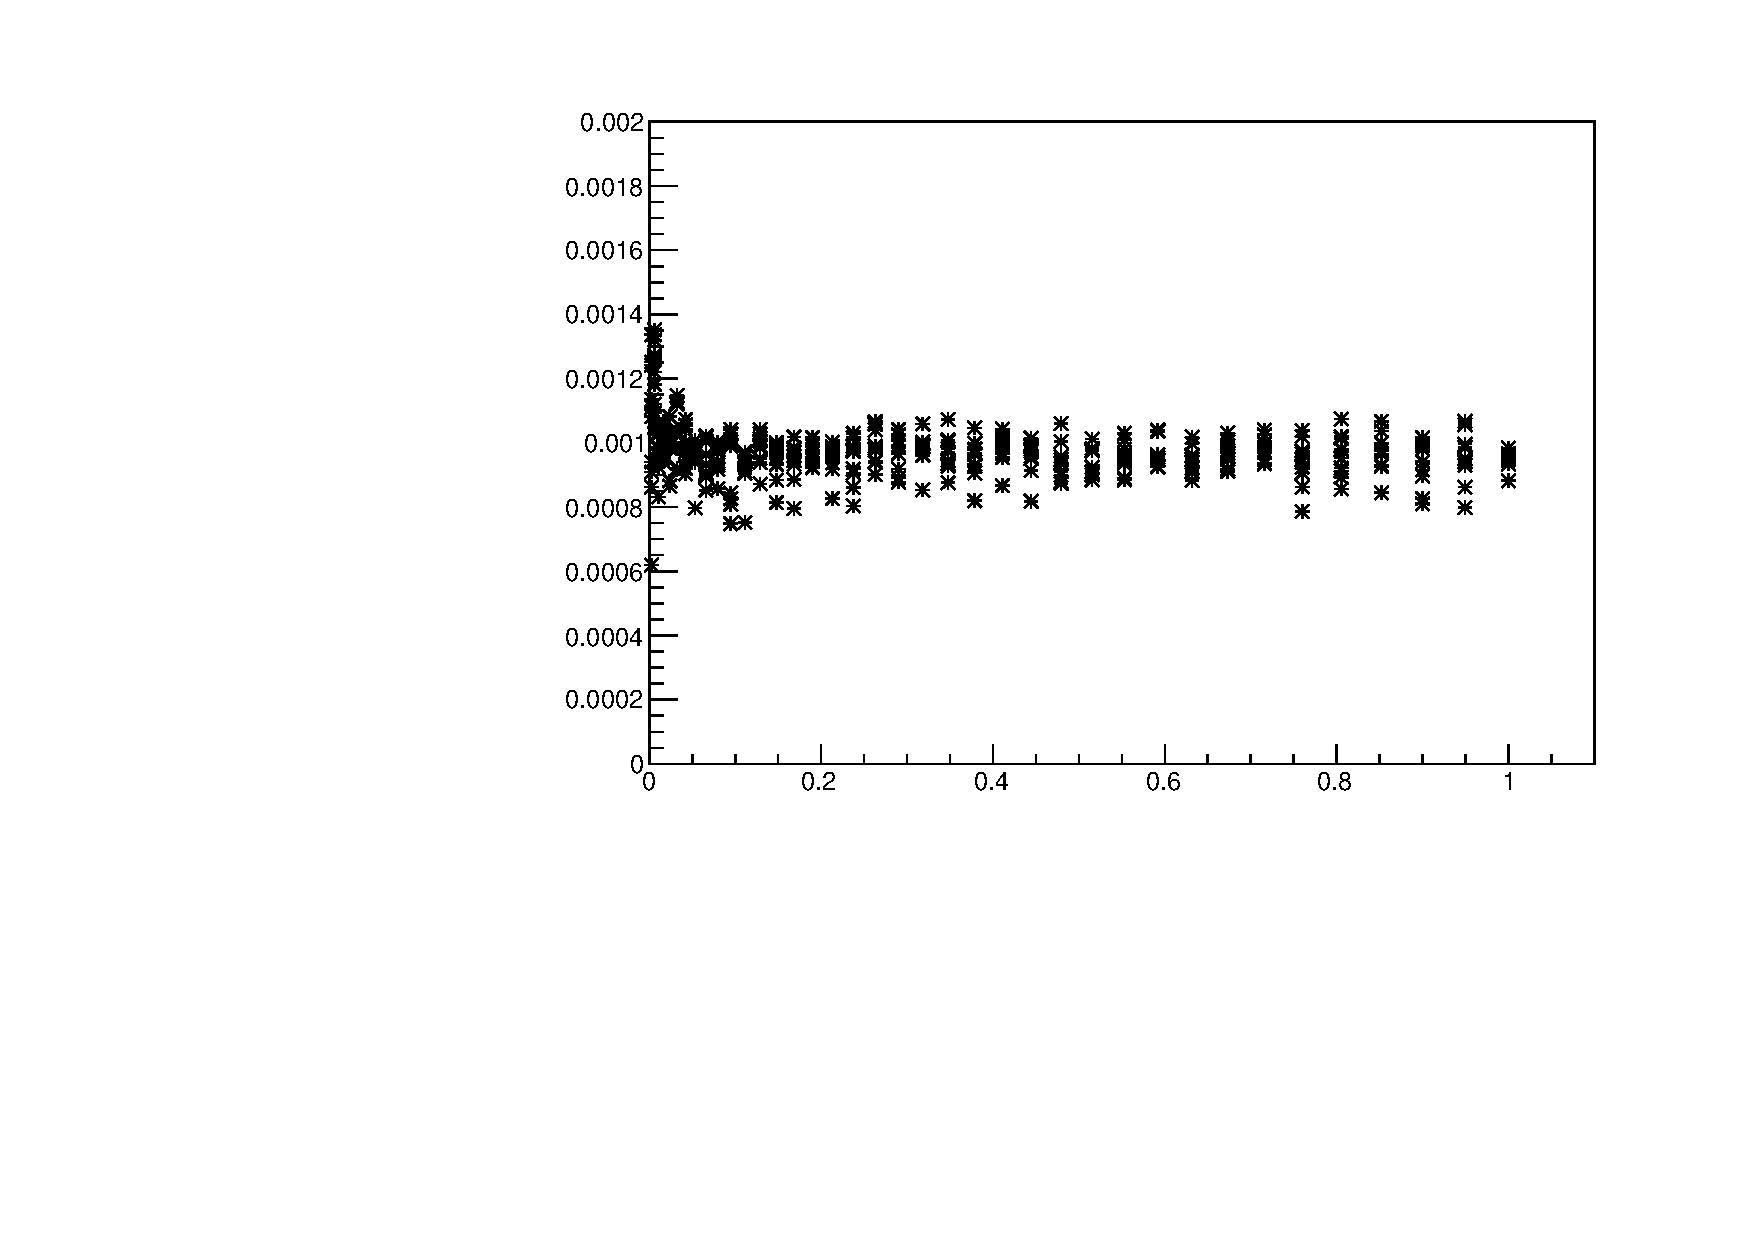
\includegraphics[width=.7\textwidth]{fig/bunny_globsmall.pdf}
\caption{random translation of $0.01$ and rotation of $3 \si{\degree}$, chosen $10$ times}
\label{fig:bunny_globsmall}
\end{figure}

\begin{figure}[H]
\centering
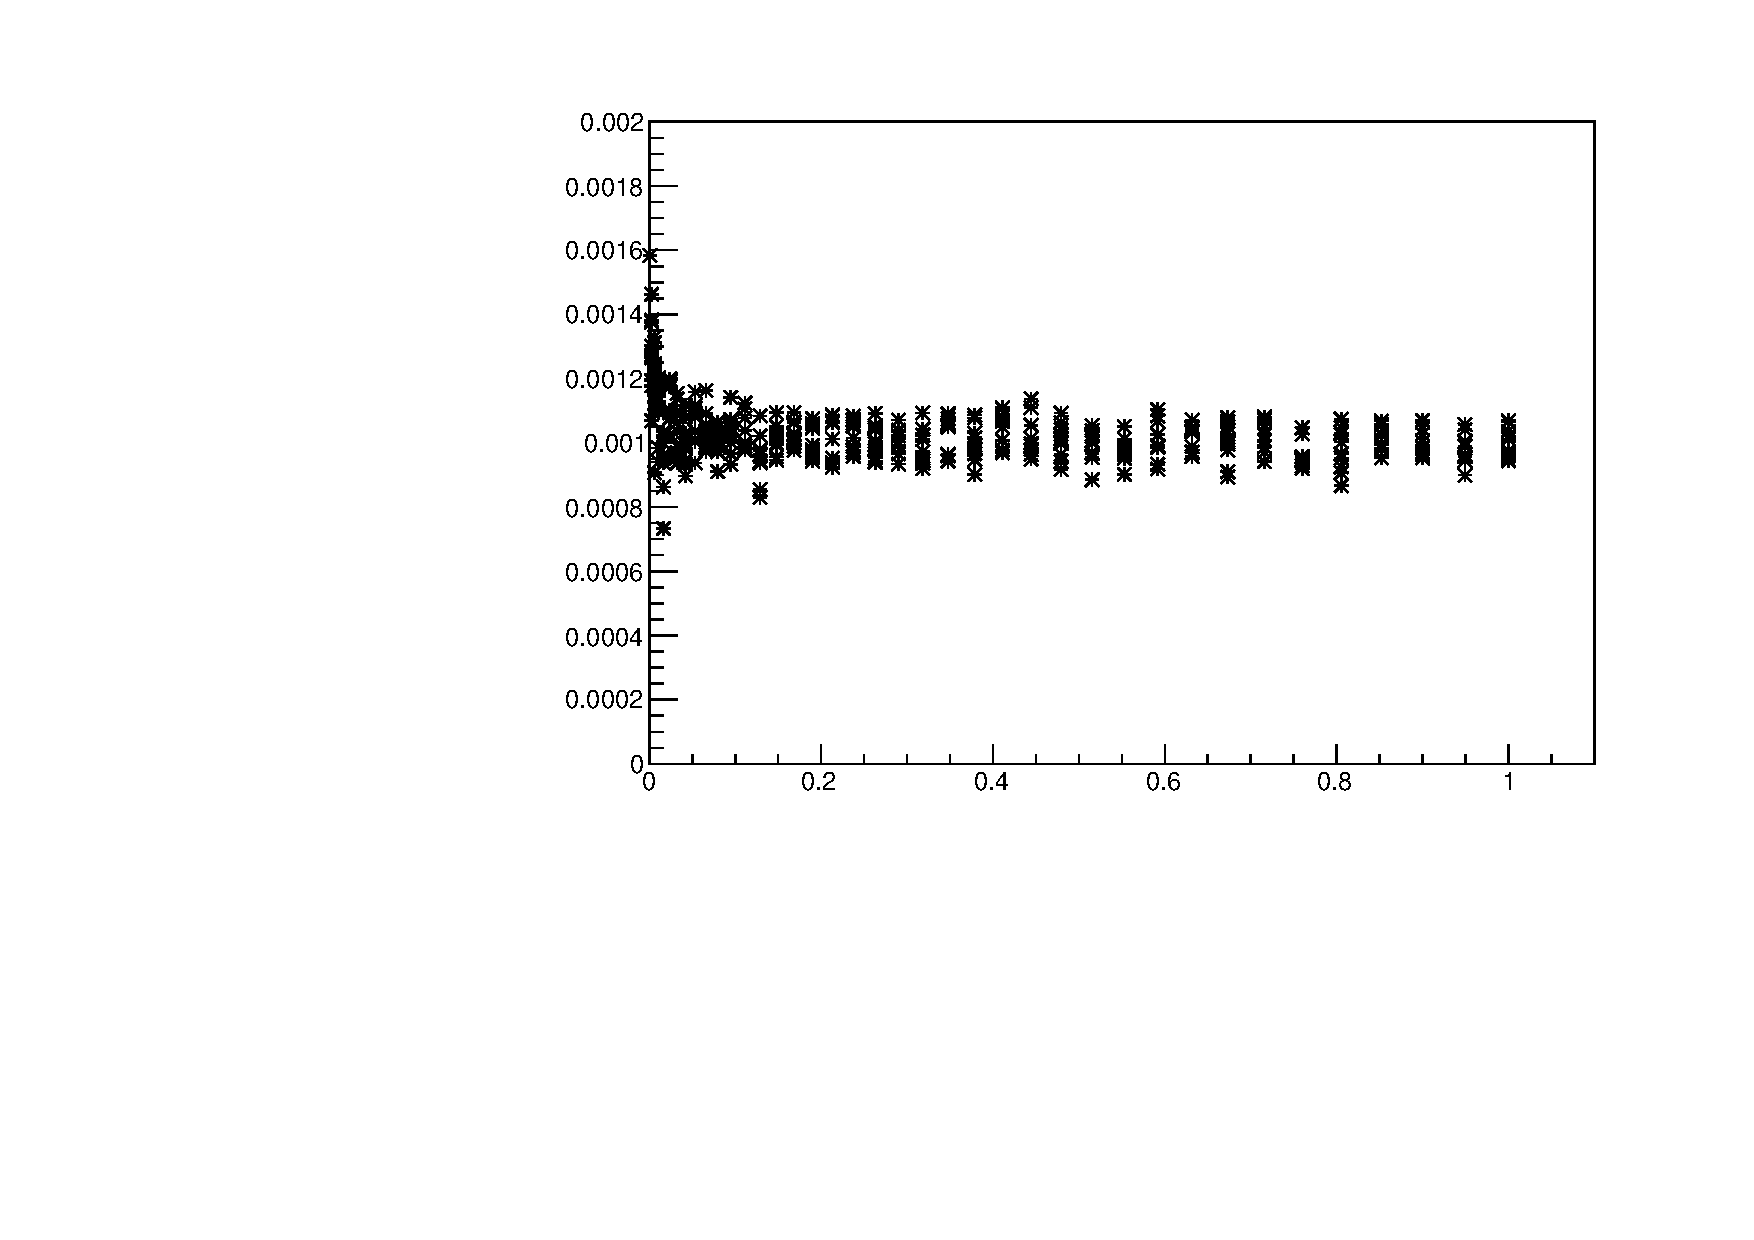
\includegraphics[width=.7\textwidth]{fig/bunny_globmed.pdf}
\caption{random translation of $0.01$ and rotation of $15 \si{\degree}$, chosen $10$ times}
\label{fig:bunny_globmed}
\end{figure}


\subsection{Evolution of registration}
This plot shows the evolution of the true error during \gls{icp} registration, for the same input point clouds. Initially the point clouds are perfectly aligned. $Q$ is randomly generated as before, results from all $60$ registration runs are superimposed.

\begin{figure}[H]
\begin{tabularx}{\textwidth}{|r|X|} \hline
Method & ICP. Select all points, closest point criterion, equal weights, no rejection, point-to-point error metric. \\ \hline
Model & Stanford Bunny model. \\ \hline
Fixed ($P$) & 50\% of model points, randomly chosen. \\ \hline
Loose ($Q$) & Starting from the other 50\%, randomly downsampled by given amount. $60$ steps. \\ \hline
Displacement & No displacement. \\ \hline
Y Axis & True error at iteration $i$. \\\hline
X Axis & Iteration step $i$. \\ \hline
\end{tabularx}
\end{figure}

\begin{figure}[H]
\centering
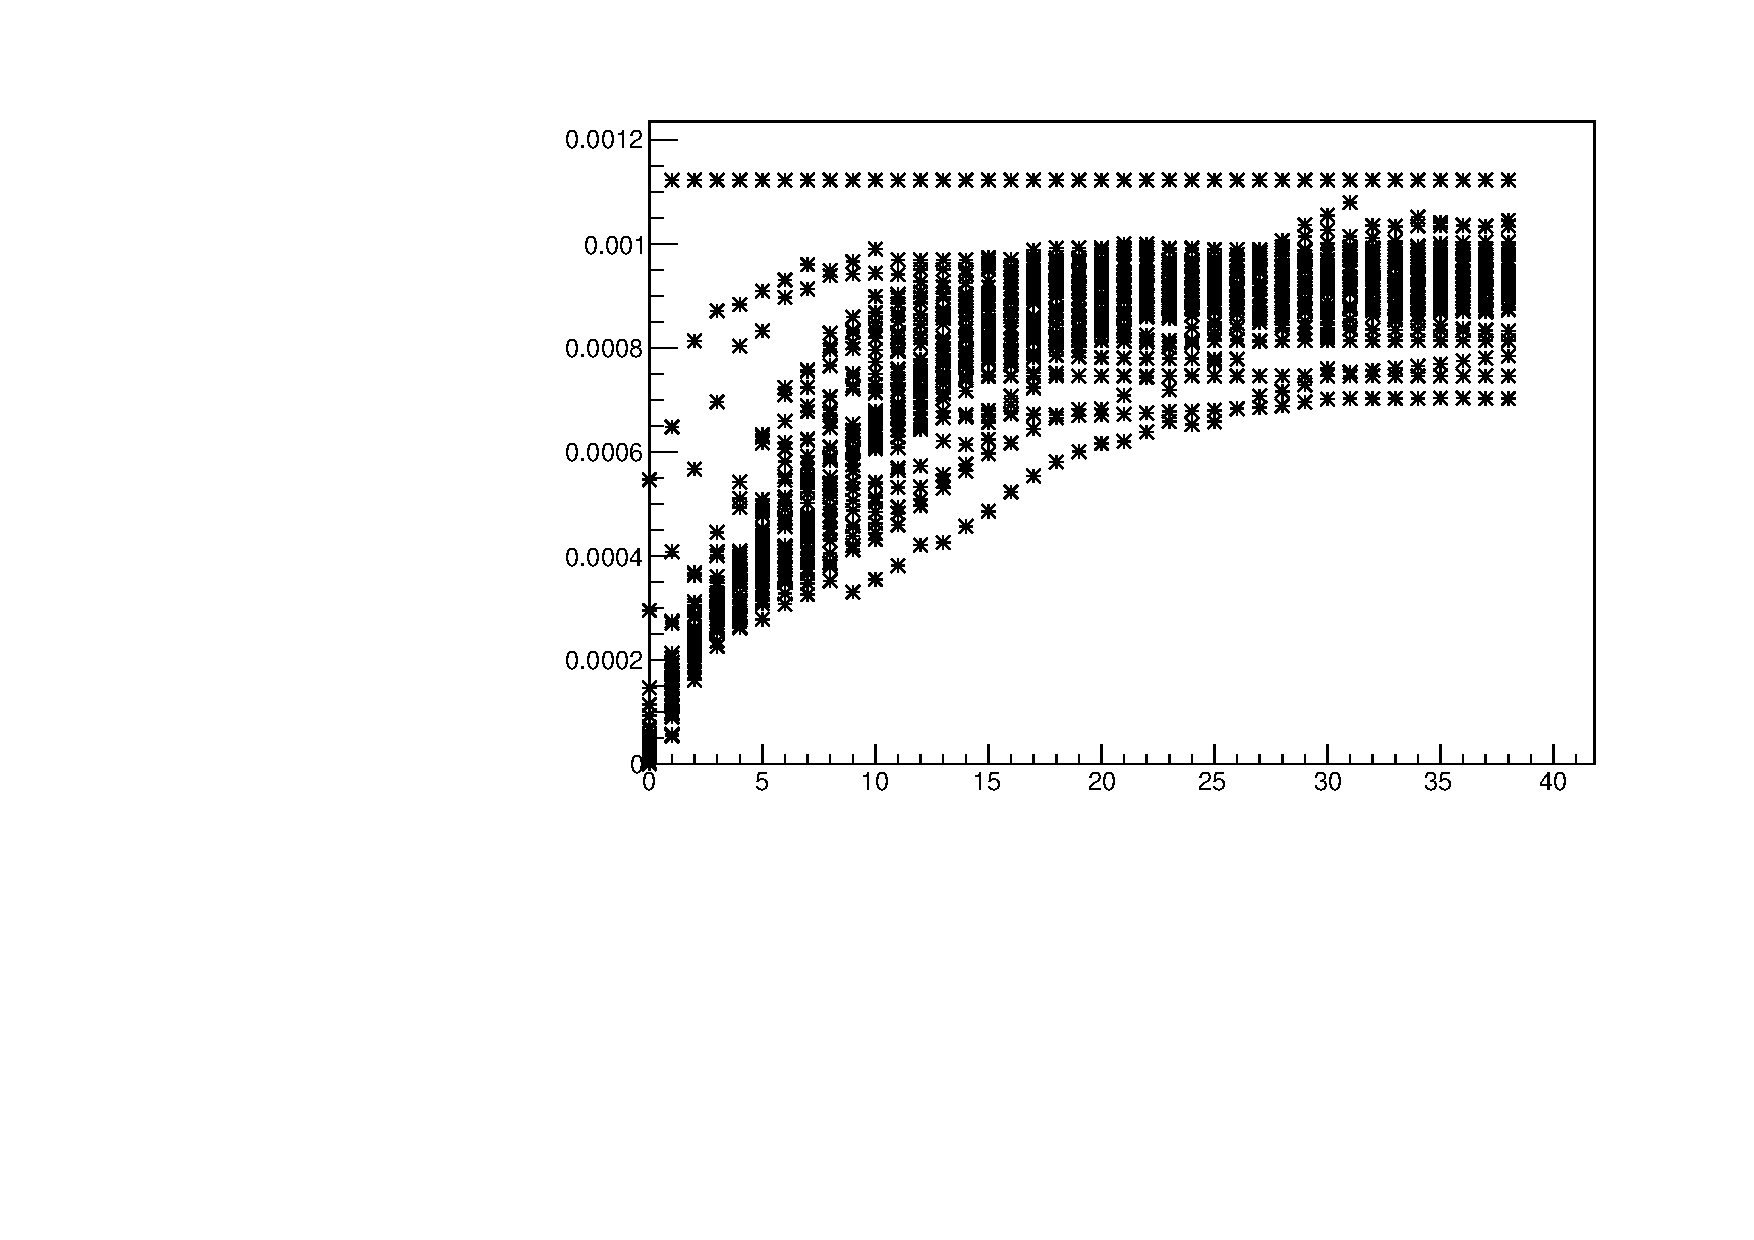
\includegraphics[width=.7\textwidth]{fig/bunny_globmin_ev.pdf}
\caption{Evolutions of true error}
\label{fig:bunny_hilo_ev}
\end{figure}



\subsection{Analysis}
Two things can be observed: The final error does not depend much on the downsampling level, and the error always converges to about $0.001$, even when $P$ and $Q$ were perfectly aligned to start with.

To define a rigid transformation, three pairs of corresponding points are sufficient as long as the three points do not lie on the same plane. (see section \ref{sec:lsq_align}) So even when $Q$ is reduced to three points the point-to-point error metric can still be minimized. \gls{ransac}-based approaches to registration, such as \gls{4pcs} are based on this.

Figure \ref{fig:bunny_hilo_ev} shows how the true error evolves during the $40$ executions of ICP on the first experiment without initial displacement. $P$ and $Q$ were generated to have no common points. When choosing the points closest to the true corresponding point instead, the error does not cancel out completely, and thus the correct alignment is no longer the global minimum of the error metric.

Figure \ref{fig:bunny_first_tcor} shows the state after the registration. $Q$ is rendered in blue color and $P$ in red. From each point $q_i \in Q$ a line segment towards the true corresponding point $q'_i$ is shown, which is not a point $p_i \in P$. On this part $Q$ has deviated towards the right from the correct alignment. The same view when $P$ and $Q$ are perfectly aligned is also shown.

\begin{figure}[h]
\centering
\hspace*{\fill}%
\begin{subfigure}{.48\textwidth}
{
	\setlength{\fboxsep}{0pt}%
	\setlength{\fboxrule}{0.5pt}%
	\fbox{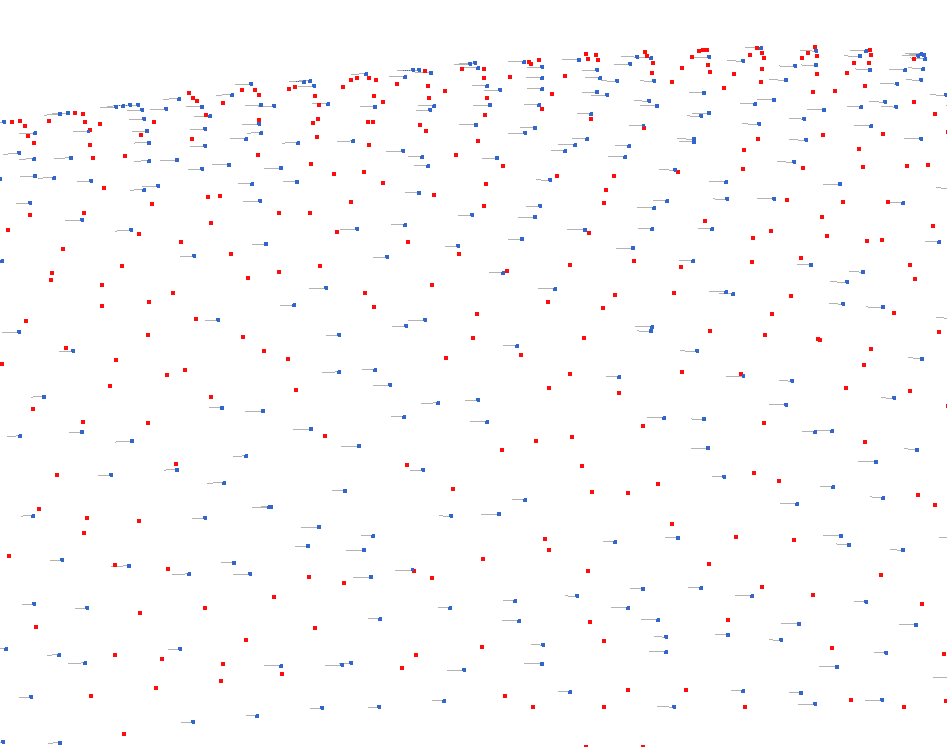
\includegraphics[width=\linewidth]{fig/bunny_first_tcor.png}}
	\caption{Result of \gls{icp} registration}
}
\end{subfigure}%
\hfill%
\begin{subfigure}{.48\textwidth}
{
	\setlength{\fboxsep}{0pt}%
	\setlength{\fboxrule}{0.5pt}%
	\fbox{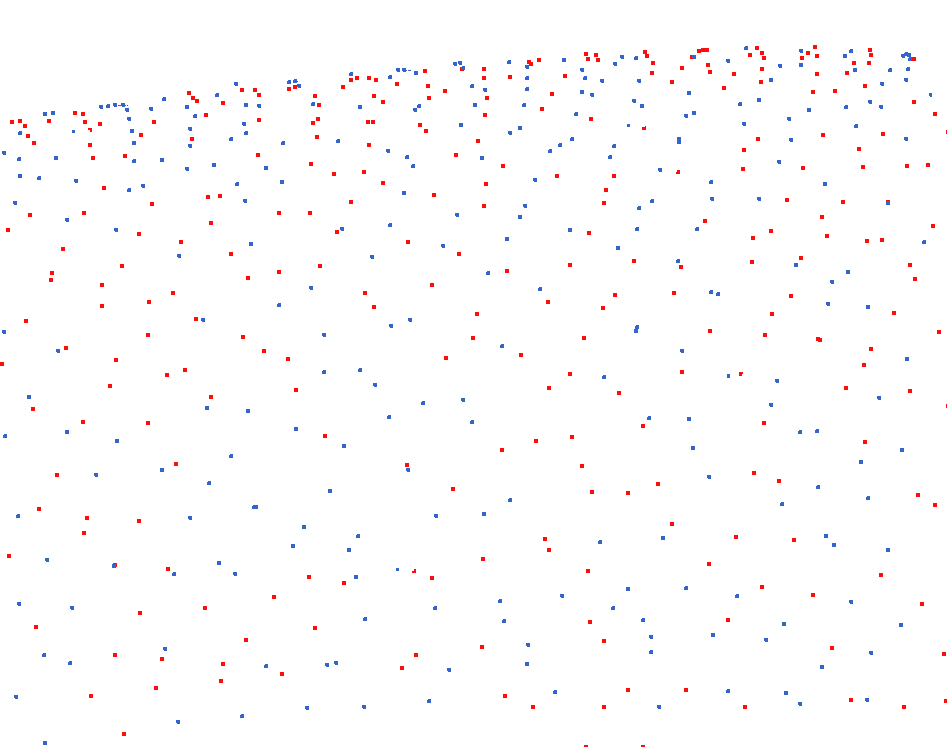
\includegraphics[width=\linewidth]{fig/bunny_first_tcor_true.png}}
	\caption{Perfect alignment}
}
\end{subfigure}%
\caption{Bunny model registered to itself, true correspondences shown}
\label{fig:bunny_first_tcor}
\end{figure}

When $\forall q_i, p_i = q'_i$, the correct alignment would be found. When $P$ and $Q$ are already aligned, $q_i = q'_i$. Figure \ref{fig:bunny_fexp_before} shows the histogram of $\|q'_i - p_i\| = \|q_i - p_i\|$ for the case when $50\%$ (or $80\%$) of the model points are taken for $P$ and the remaining for $Q$, and no additional downsampling is applied.

\begin{figure}[H]
\centering
\begin{subfigure}{.5\textwidth}
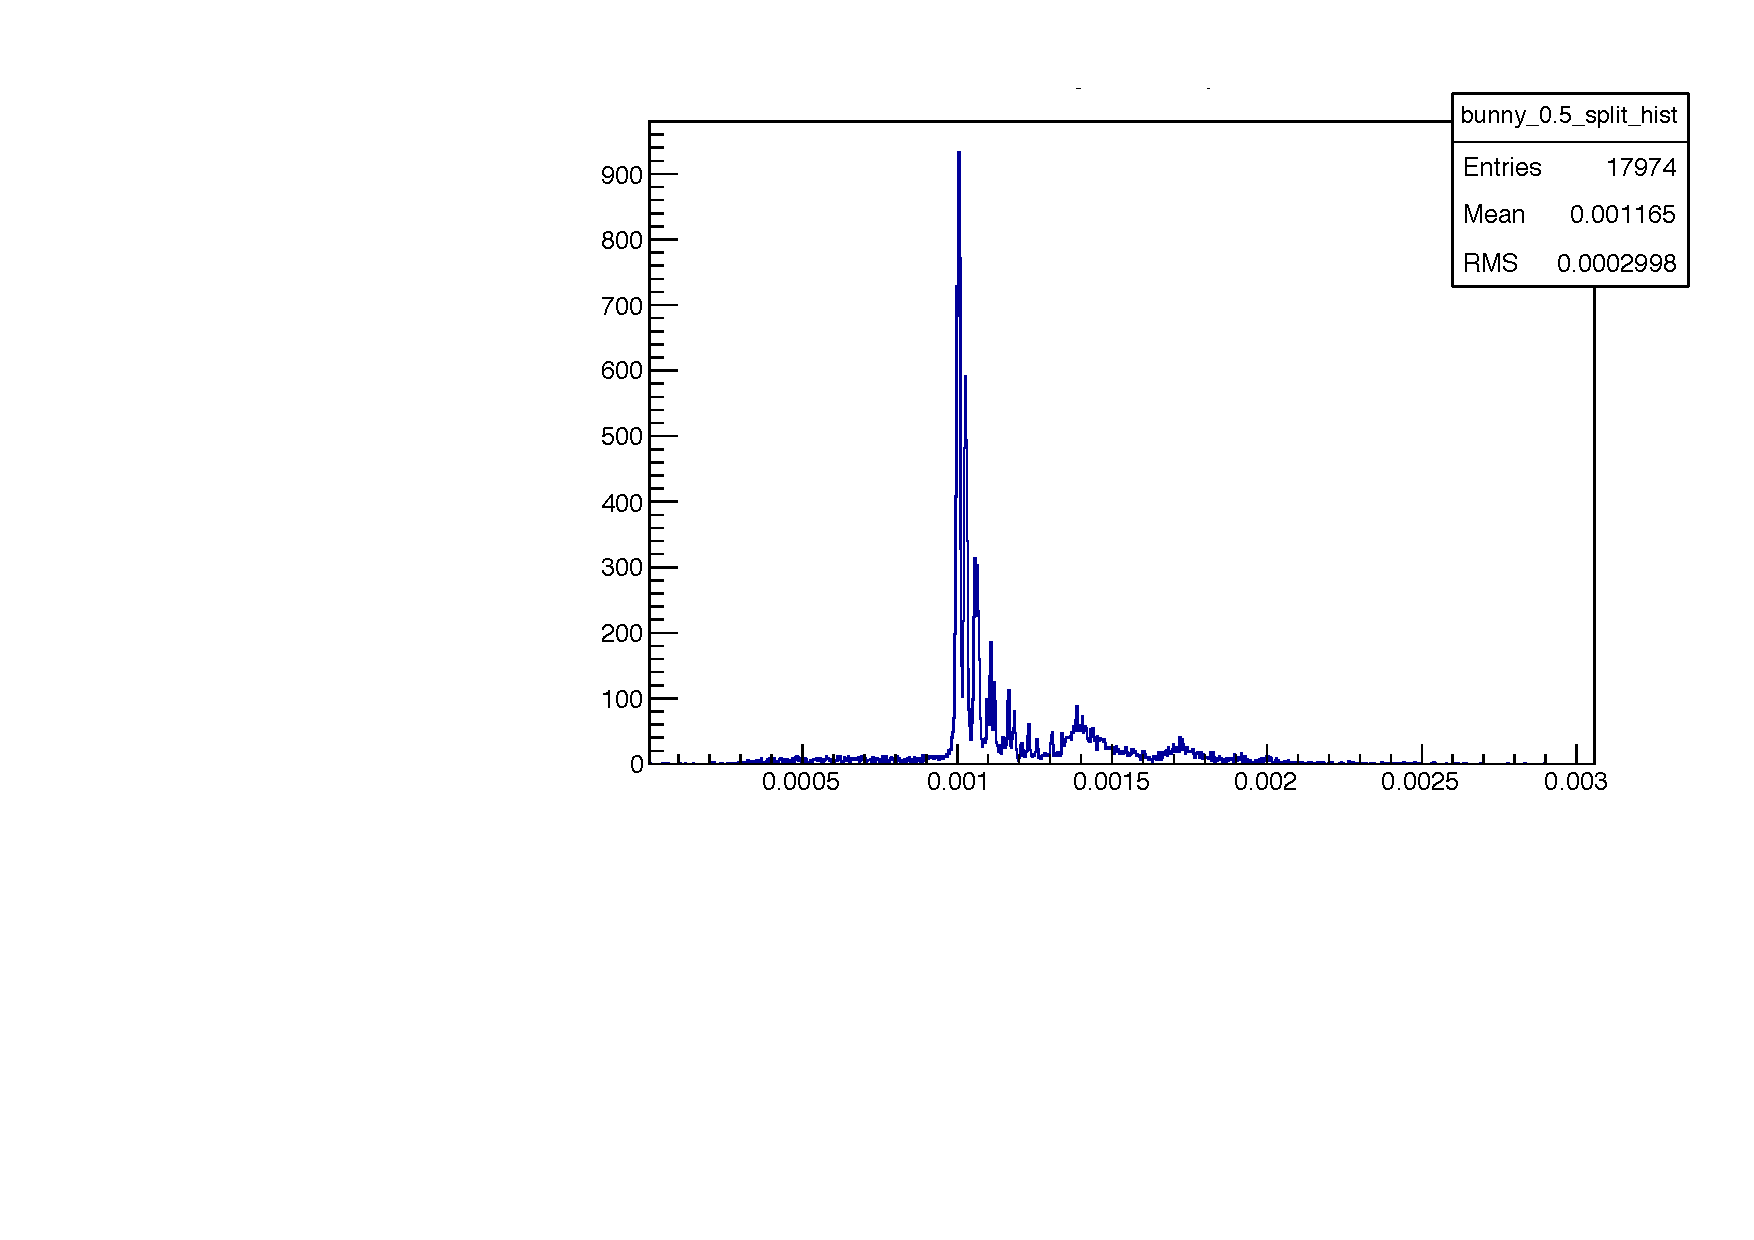
\includegraphics[width=\linewidth]{fig/bunny_05_split.pdf}
\end{subfigure}%
\begin{subfigure}{.5\textwidth}
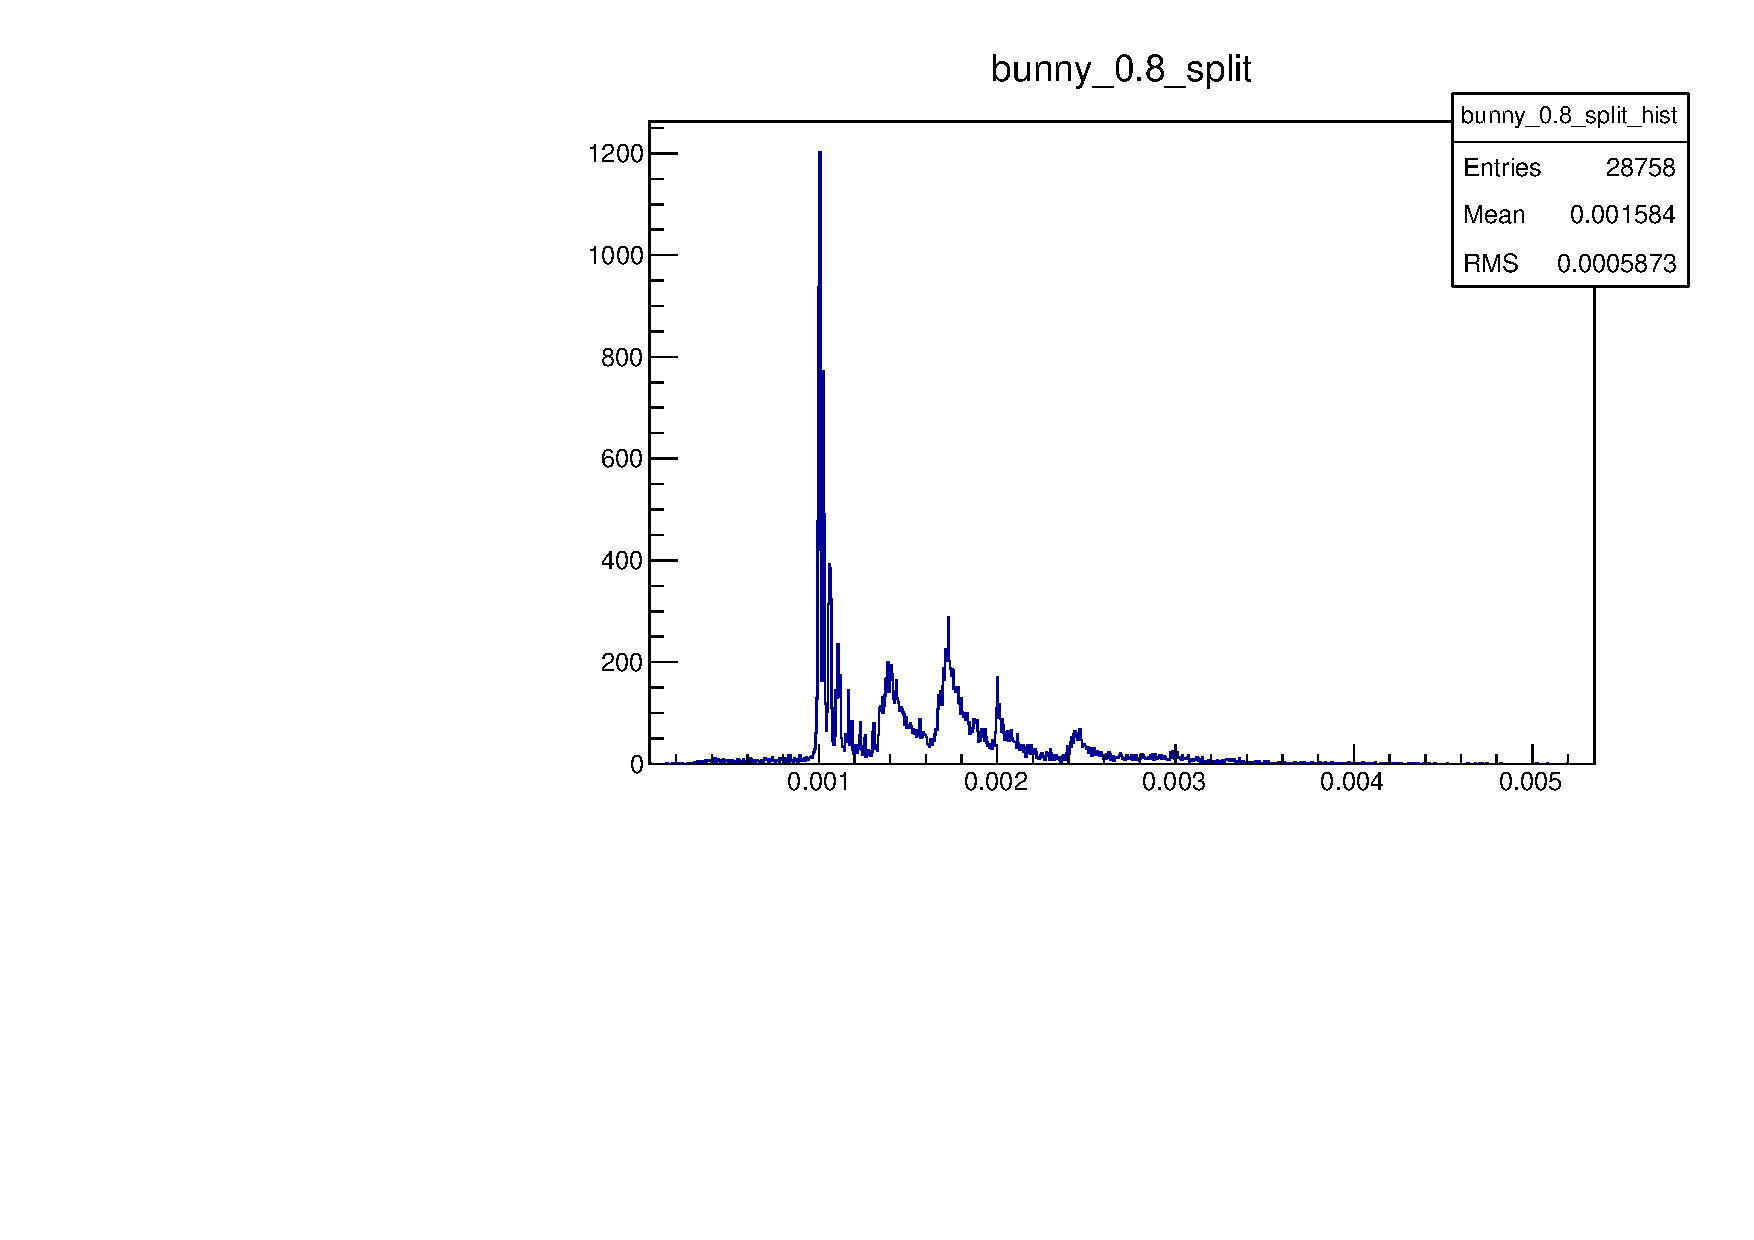
\includegraphics[width=\linewidth]{fig/bunny_08_split.pdf}
\end{subfigure}
\caption{Histograms of $\|q_i - p_i\|$ for 50\% and 80\% split}
\label{fig:bunny_fexp_before}
\end{figure}

In both cases, $\| q - p \| \approx 0.001$ is a mode in the distribution. Smaller values are infrequent. Additional spikes occur for some values above $0.001$. 

The reason is that for the original Bunny point clouds, the points are evenly distributed on the surface on an approximatively square grid, with a mean distance of about $0.001$ between adjacent points, as seen in the close-up view in figure \ref{fig:bunny_grid_closeup}. Figure \ref{fig:bunny_closest} shows a histogram made by taking from each point $p$ on the Bunny point cloud $B$, the closest point $p' \in B$ with $p' \neq p$. In the closest point histograms from $Q$ to $P$, any point that is in $Q$ is missing in $P$ and hence the closest point is often the one at a distance of $0.001$. Some instances appear where this point is not in $P$ either, so the closest point is further. This explains the spike at $0.002$. The other spikes occur when the closest point is in a diagonal direction on the grid. This ``grid'' is approximate and the surface is embedded in a non planar way in 3D space, so most samples do not fall exactly in one of these spikes.

For the true correspondences, the histogram would be a single spike at $\|p_i - q'_i\| = 0$. 

\begin{figure}[h]
\centering
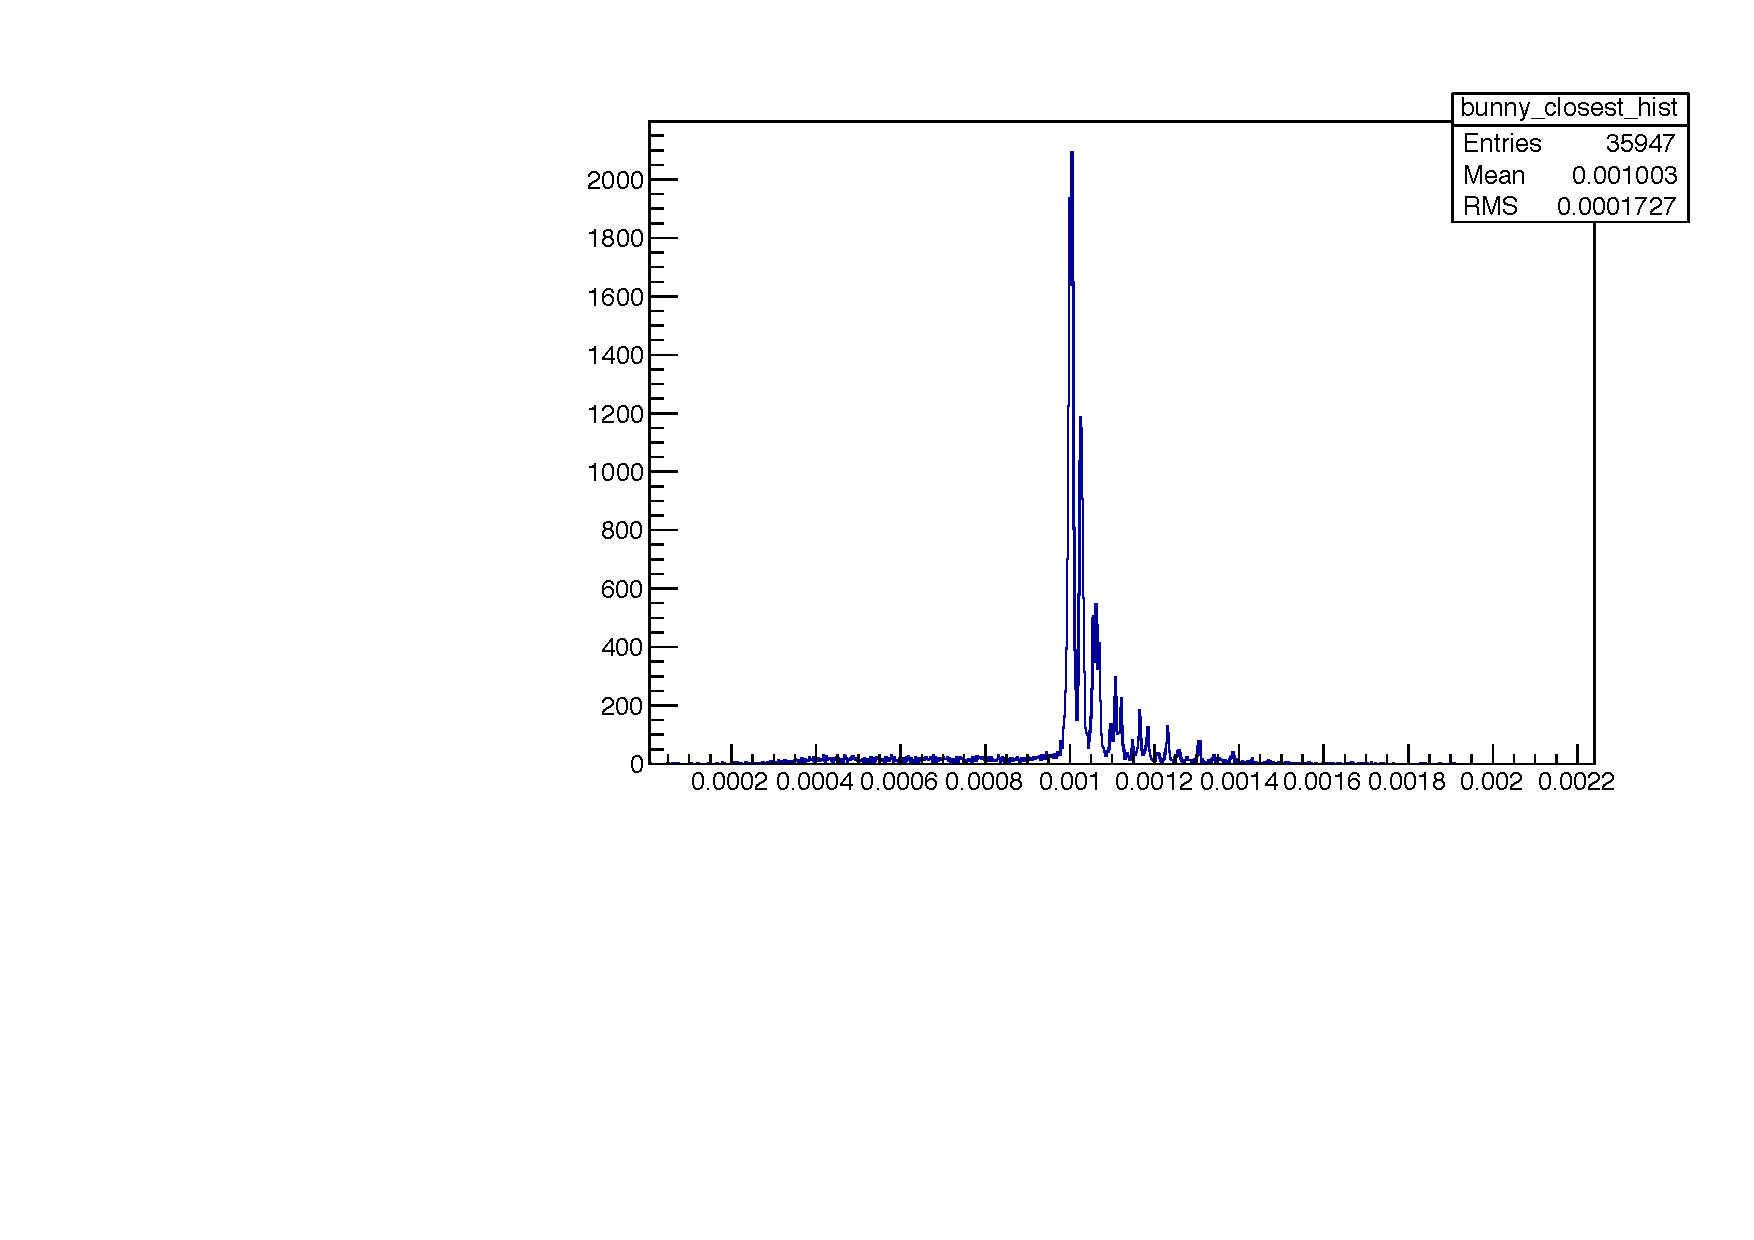
\includegraphics[width=.5\linewidth]{fig/bunny_closest.pdf}
\caption{Nearest neighbor distance histogram on Bunny point cloud}
\label{fig:bunny_closest}
\end{figure}


\subsection{Sphere experiment}
A similar experiment was run on artificially generated sphere point clouds, where the points are randomly dispersed on the sphere surface at a given density. Both the number of points on the fixed and on the loose point clouds are varied. Because of the random dispersion they generally never coincide perfectly. 

The X-axis on the plot shows the \emph{maximal} number of points, of the loose point clouds and of the fixed point cloud. Initially the point clouds are perfectly aligned, and they deviate from that alignment during \gsl{icp} registration.

It can be seen that the mean error, and its variance are slightly larger when fewer points are involved, because the point dispersion is less dense on the surfaces, and so the nearest neighbor distances get greater. However, because the points here are dispersed randomly, there is already a high variance in the nearest neighbor distances, as will be shown later.

\begin{figure}[H]
\begin{tabularx}{\textwidth}{|r|X|} \hline
Method & ICP. Select all points, closest point criterion, equal weights, no rejection, point-to-point error metric. \\ \hline
Model & Artificially generated sphere point cloud with random point dispersion. \\ \hline
Fixed ($P$) & Randomly chosen number of points from $0$ to $50000$. $30$ steps. \\ \hline
Loose ($Q$) & Randomly chosen number of points from $0$ to $50000$. $30$ steps. \\ \hline
Displacement & No displacement. \\ \hline
Y Axis & True error, after $40$ iterations. \\\hline
X Axis & Maximum of number of points in $Q$ and number of points in $P$. \\ \hline
\end{tabularx}
\end{figure}

\begin{figure}[H]
\centering
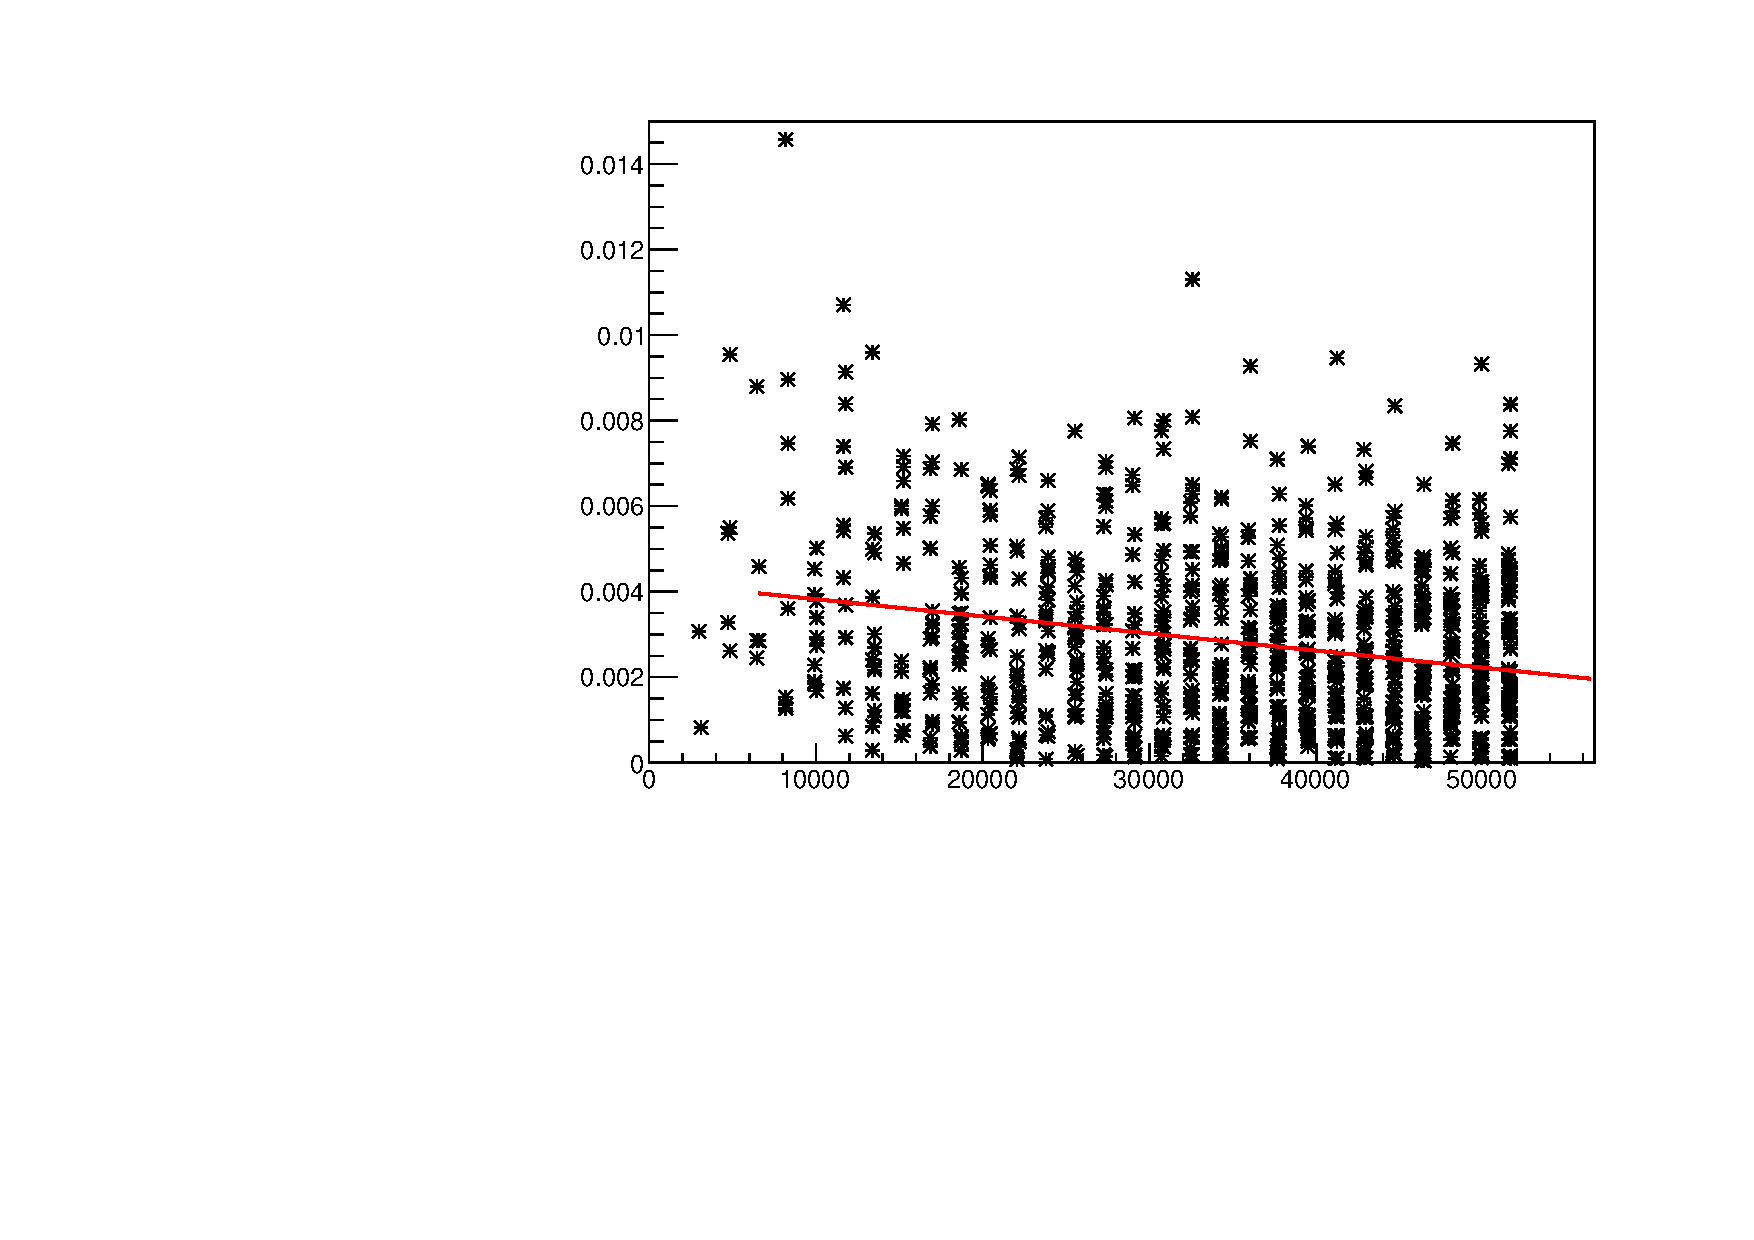
\includegraphics[width=.7\textwidth]{fig/sphere_icp.pdf}
\caption{Sphere experiment results}
\end{figure}


\subsection{Different view points}
Another experiment was run to test \gls{icp}'s sensitivity to occlusion caused by differing camera angles. A relief model as described in \ref{sec:relief} is used. The fixed and loose point clouds are both generated by generating a projected range image of it, with a camera placed at a higher altitude, looking down on the relief, and placed at an angle $\theta$ relative to the Y axis. For both the loose and the fixed point cloud these angles $\theta_{\text{fixed}}$ and $\theta_{\text{loose}}$ are independently varied from $0$ to $2 \pi$.

When $\theta_{\text{fixed}} = \theta_{\text{loose}}$ both point clouds feature the relief looked at from the same view point, thus there are no occluded parts from one point clouds relative to the other. As the difference gets greater the overlapping area gets smaller.

An example is shown on figures \ref{fig:relief_dproj}. On the first figure both point clouds are projected from the same view point. They are cropped to have different bounds, like point clouds from real scans would have. On the second figure the view point of the red point cloud is different.

Initially the $P$ and $Q$ are perfectly aligned, and then \gls{icp} is run. The final true error is recorded. It can be seen that as the overlap gets smaller, \gls{icp} tends to converge towards an alignment that lays further off the true tranformation, even when the point clouds were perfectly aligned to start with.

Thus the global minimum of the error metric minimized by point-to-point \gls{icp} diverges from the true transformation.

\begin{figure}[h]
\centering
\begin{subfigure}{.5\textwidth}
	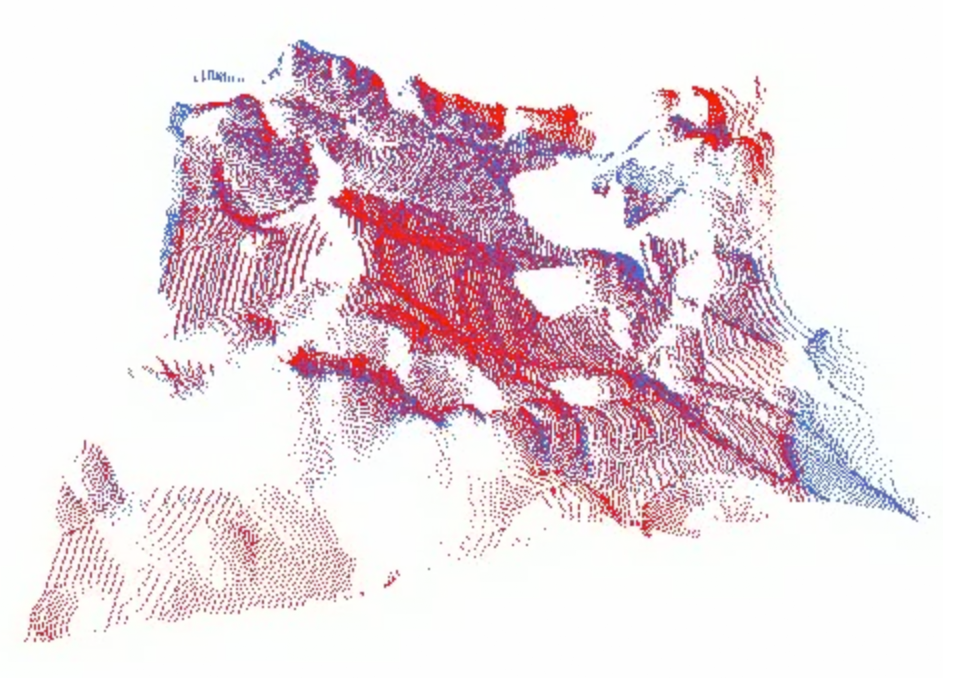
\includegraphics[width=\linewidth]{fig/relief_dproj_1.png}
	\caption{Same view point}
\end{subfigure}%
\begin{subfigure}{.5\textwidth}
	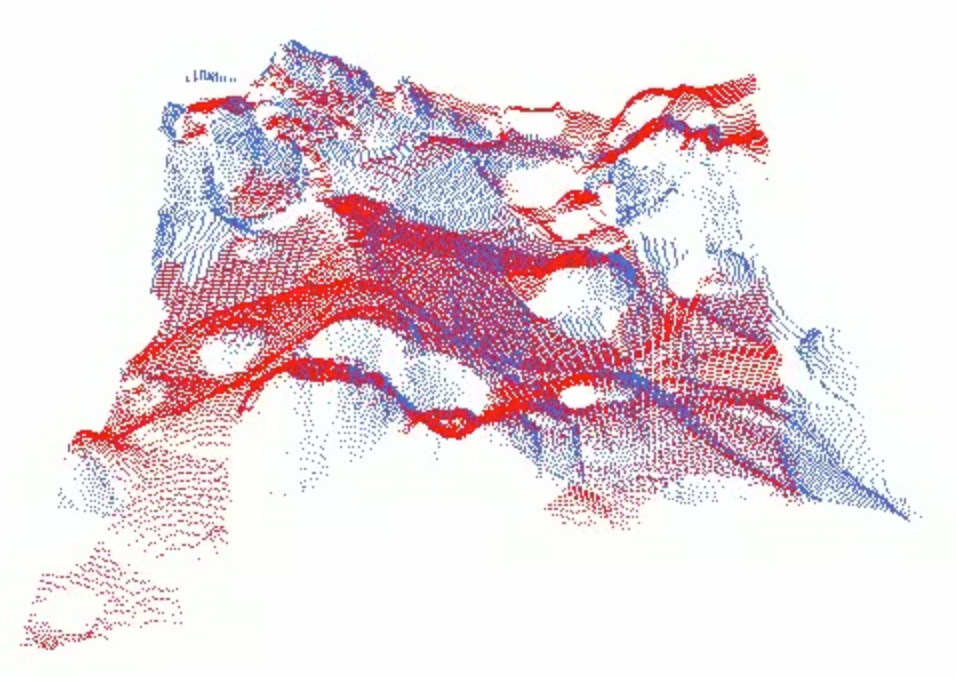
\includegraphics[width=\linewidth]{fig/relief_dproj_2.png}
	\caption{Different view points}
\end{subfigure}
\caption{Aligned relief point clouds, projected from different angles}
\label{fig:relief_dproj}
\end{figure}

\begin{figure}[H]
\begin{tabularx}{\textwidth}{|r|X|} \hline
Method & ICP. Select all points, closest point criterion, equal weights, no rejection, point-to-point error metric. \\ \hline
Model & Relief point cloud, projected with occlusion from camera placed at angle looking down on relief. \\ \hline
Fixed ($P$) & Point cloud of relief with camera angle varying in $[0, 2 \pi]$ around relief. $20$ steps. \\ \hline
Loose ($Q$) & Point cloud of relief with camera angle varying in $[0, 2 \pi]$ around relief. $20$ steps. \\ \hline
Displacement & No displacement. \\ \hline
Y Axis & True error, after $40$ iterations. \\\hline
X Axis & Angle between Fixed and Loose camera positions. \\ \hline
\end{tabularx}
\end{figure}
\begin{figure}[H]
\centering
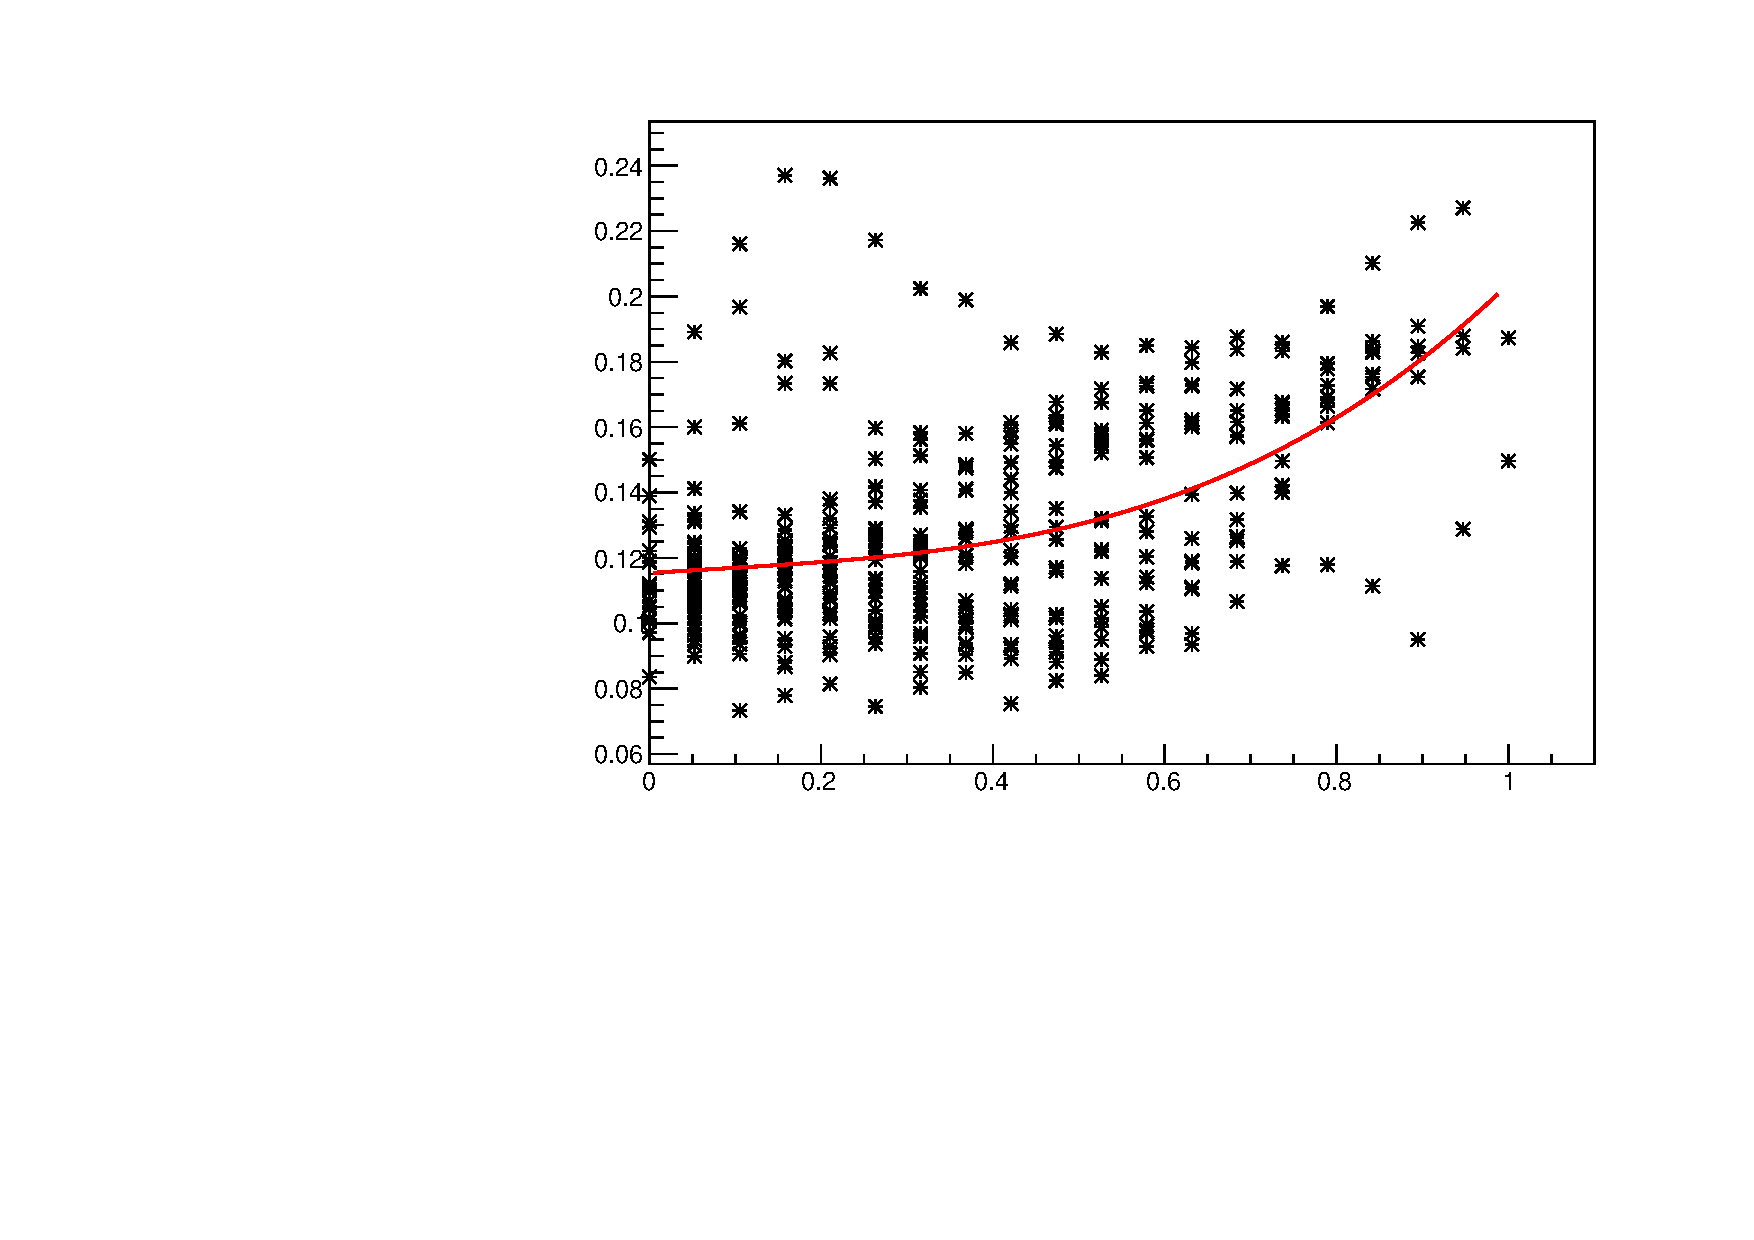
\includegraphics[width=.7\textwidth]{fig/relief_dproj.pdf}
\caption{Different view-points experiment results}
\end{figure}


\subsection{Conclusion}
It can be concluded that the accuracy of registration that one can hope to attain with the \gls{icp} point-to-point error metric is limited by the density with which points are dispersed on the object surfaces. For the Bunny point cloud the final \emph{true error} after \gls{icp} registration tends to be off in average by the side length of the square grid which the points form.

When a much higher resolution version of the model should be registered with it, this remaining error becomes significant.

Also, the accuracy is reduced when the point clouds are projected from more different view-points, because their overlap gets lower.


\section{Instability of ICP error metric}
The experiments show that the point-to-point error metric used by \gls{icp} is unstable, in the sense that its accuracy deteriorates when one point cloud has lower resolution, and when they have low overlap due to different camera view poses.

Figure \ref{fig:relief_err} is a visualization of the \emph{mean absolute error} with closest-point correspondences, taken on a relief model. As explained before the curves show the value of $e(\matr{\hat{M}})$ for randomly chosen one-dimensional cross-sections of the rigid transformation space, such that $\matr{\hat{M}}$ is the true transformation $\matr{M}$ at $x = 0$. Therefore all the curves on the plots intersect at $x = 0$. An accurate error metric would have its global minimum at $x = 0$ and no local minima.

On these cross sections $\matr{\hat{M}}$ deviates from $\matr{M}$ by a maximum of $0.003$ translation length and $0.3\si{\degree}$ rotation angle. The relief model has a width of $5$ by comparison.

\begin{figure}[H]
\centering
\begin{subfigure}{.33\textwidth}
	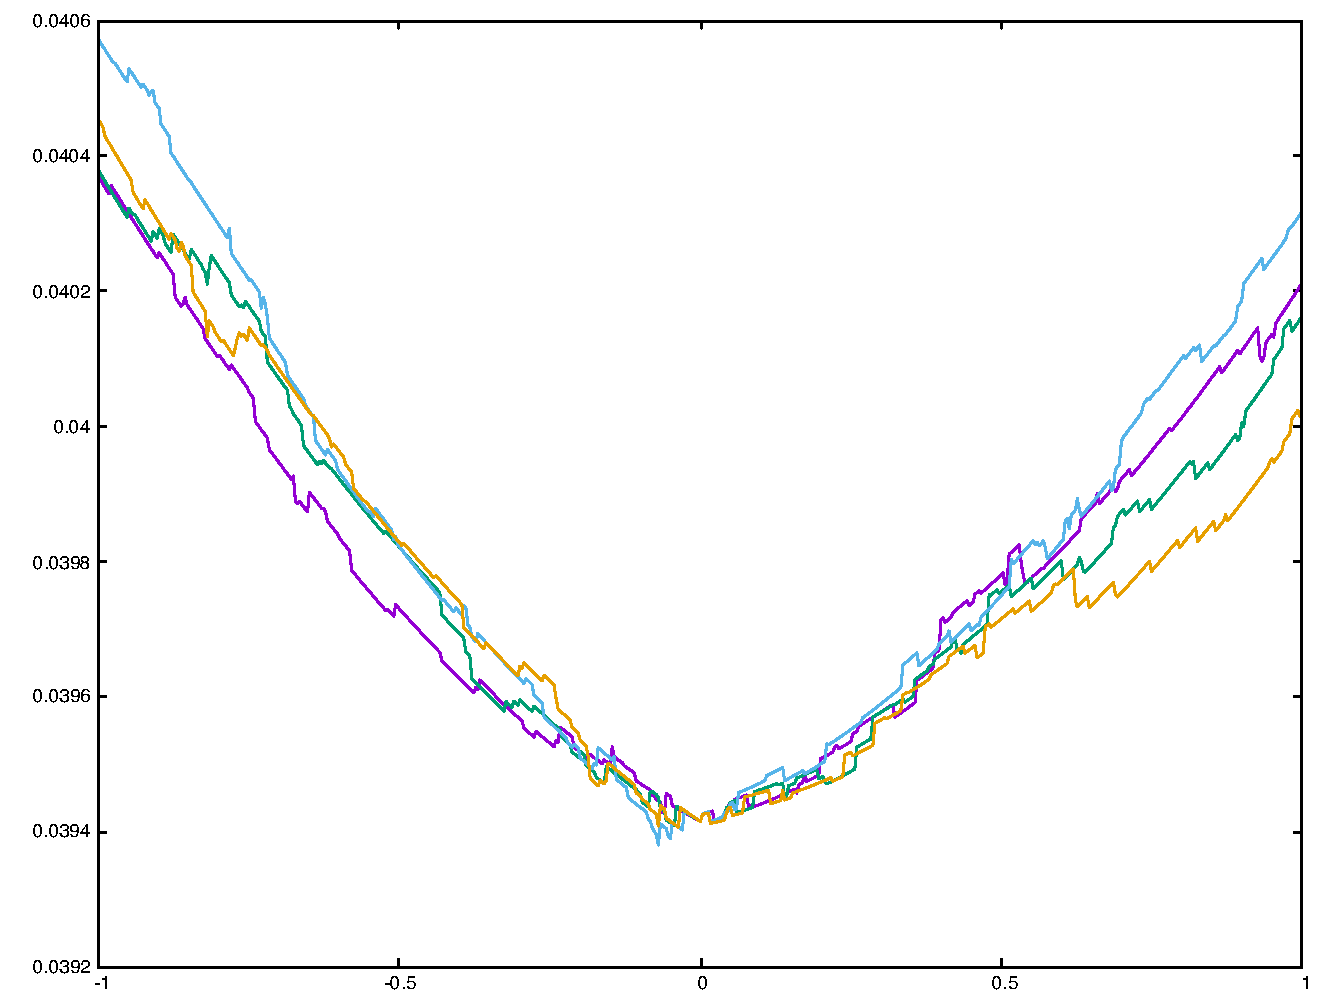
\includegraphics[width=\linewidth]{fig/relief_same_err.pdf}
	\caption{Same}
\end{subfigure}%
\begin{subfigure}{.33\textwidth}
	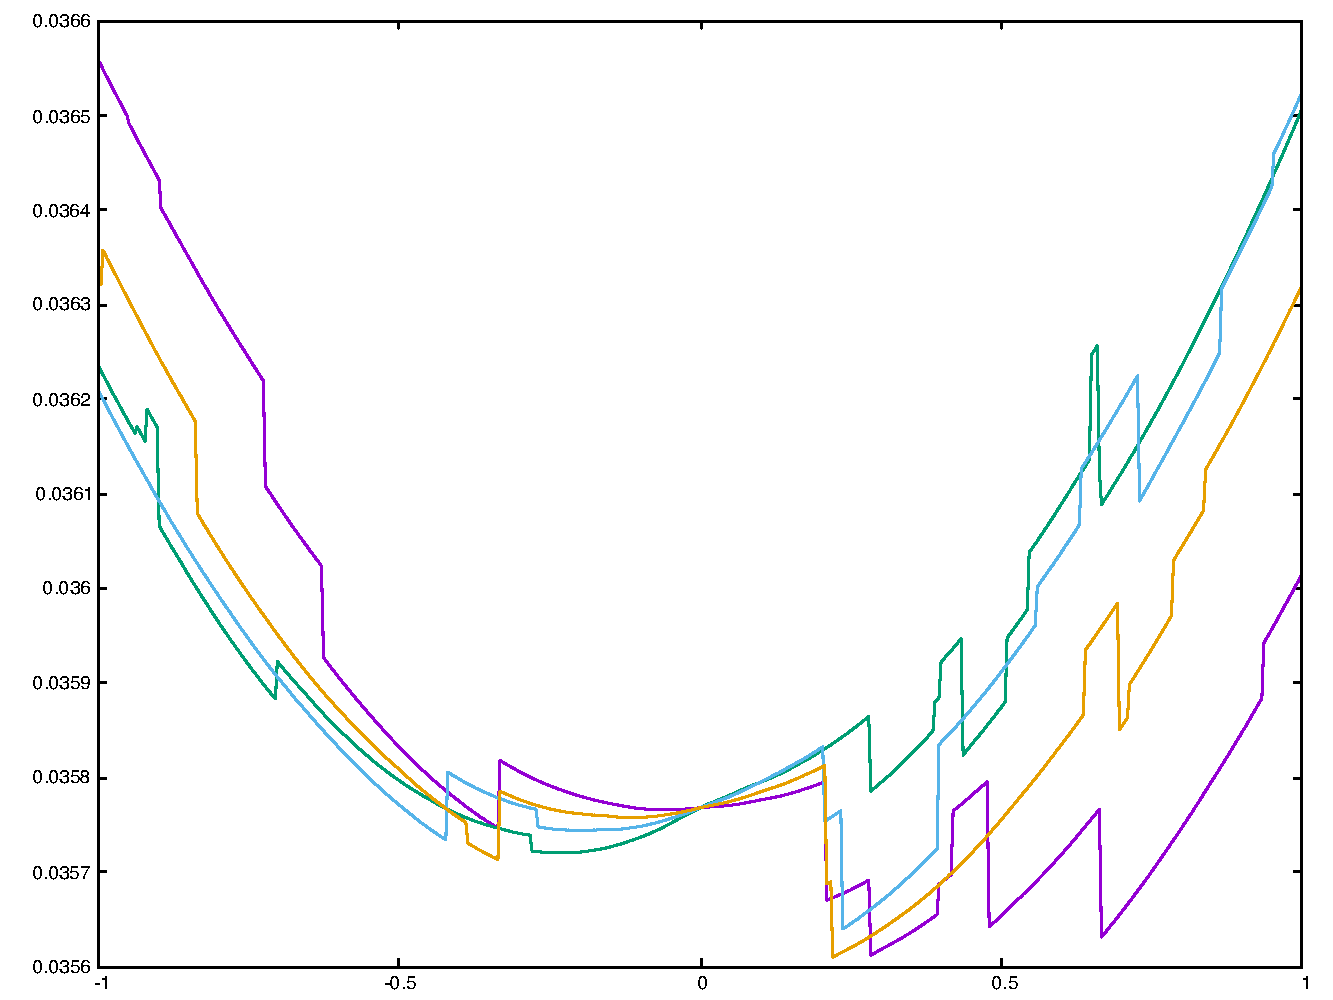
\includegraphics[width=\linewidth]{fig/relief_hilo_err.pdf}
	\caption{Different resolution}
\end{subfigure}
\begin{subfigure}{.33\textwidth}
	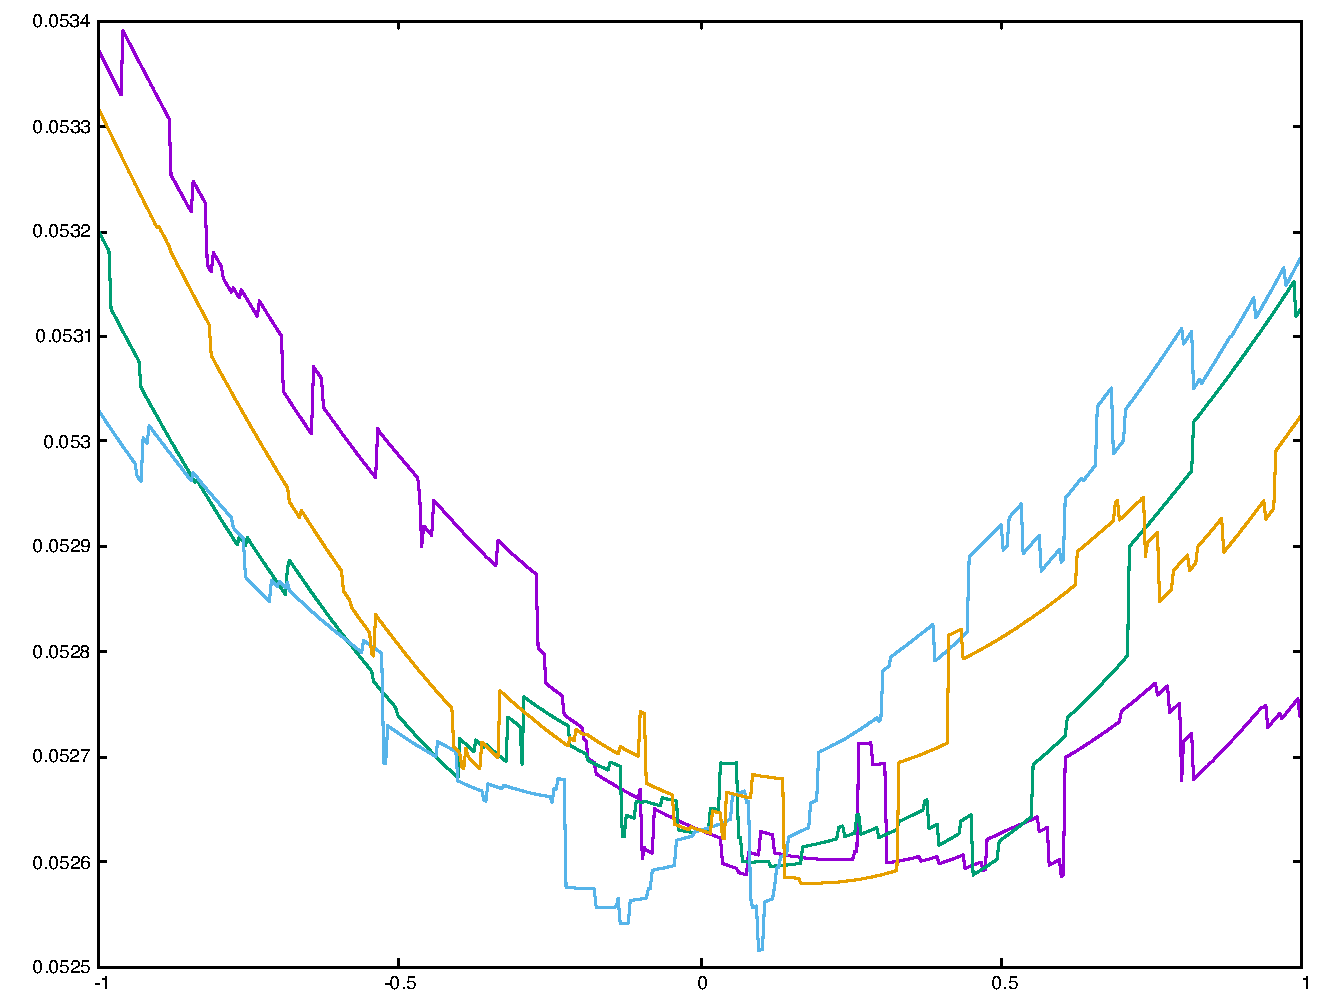
\includegraphics[width=\linewidth]{fig/relief_dproj_err.pdf}
	\caption{Different view-point}
\end{subfigure}
\caption{Mean absolute error metric visualization with closest-point criterion}
\label{fig:relief_err}
\end{figure}

In the first plot the fixed and loose point cloud have approximately the same resolution and total overlap, whereas in the other two cases their resolution or view-point has been altered like in the experiments.

It can be seen that in those two cases, $\matr{M}$ is no longer the global minimum, and so \gls{icp} converges to another transformation as it did in the experiment runs. In the next chapters the attempt is made to develop an error metric that remains more stable.
